\documentclass[11pt,a4paper]{article}
\usepackage[top=3cm, bottom=2cm, left=2cm, right=2cm]{geometry}
\usepackage[utf8]{inputenc}
\usepackage{amsmath, amsfonts, amssymb}
\usepackage{siunitx}
\usepackage[brazil]{babel}
\usepackage{graphicx}
\usepackage[margin=10pt,font={small, it},labelfont=bf, textfont=it]{caption}
\usepackage[dvipsnames, svgnames]{xcolor}
\DeclareCaptionFont{MediumOrchid}{\color[svgnames]{MediumOrchid}}
\usepackage[pdftex]{hyperref}
\usepackage{natbib}
\bibliographystyle{plainnat}
\bibpunct{\textcolor{MediumOrchid}{\textbf{[}}}{\textcolor{MediumOrchid}{\textbf{]}}}{,}{s}{}{}
\usepackage{color}
\usepackage{footnote}
\usepackage{setspace}
\usepackage{booktabs}
\usepackage{multirow}
\usepackage{subfigure}
\usepackage{fancyhdr}
\usepackage{leading}
\usepackage{indentfirst}
\usepackage{wrapfig}
\usepackage{mdframed}
\usepackage{etoolbox}
\usepackage[version=4]{mhchem}
\usepackage{enumitem}
\usepackage{caption}
\usepackage{titlesec}
\usepackage{tcolorbox}
\usepackage{tikz}
\usepackage{LobsterTwo}
\usepackage[T1]{fontenc}
\usepackage{fontspec}
\usepackage{txfonts}
\usepackage[bottom]{footmisc}
\tcbuselibrary{skins,breakable}
\sisetup{output-decimal-marker={.}}

\makeatletter
\def\footnoterule{\kern-3pt\color{MediumOrchid}\hrule\@width0.6\textwidth height 0.8pt\kern2.6pt}
\makeatother

\renewcommand{\footnotelayout}{\itshape\color{MediumOrchid}}

\AtBeginEnvironment{equation}{\fontsize{13}{16}\selectfont}


\titleformat{\section}{\LobsterTwo\huge\color{CarnationPink}}{\thesection.}{1em}{}
\titleformat{\subsection}{\LobsterTwo\huge\color{CarnationPink}}{\thesubsection}{1em}{}
\titleformat{\subsubsection}{\bf\LobsterTwo\Large\color{MediumOrchid}}{\thesubsubsection}{1em}{}


\DeclareCaptionLabelFormat{figuras}{\textcolor{DarkTurquoise}{Figura \arabic{figure}}}
\captionsetup[figure]{labelformat=figuras}

\makeatletter
\renewcommand\tagform@[1]{\maketag@@@{\color{CarnationPink}(#1)}}
\makeatother

\renewcommand{\theequation}{Eq. \arabic{equation}}
\renewcommand{\thefigure}{Fig. \arabic{figure}}
\renewcommand{\thesection}{\textcolor{CarnationPink}{\arabic{section}}}

\setlist[itemize]{label=\textcolor{CarnationPink}{$\blacksquare$}}

\setlist[enumerate]{label=\textcolor{CarnationPink}{\arabic*.}, align=left, leftmargin=1.5cm}


\newcounter{exemplo}

\NewDocumentEnvironment{exemplo}{ O{} }{%
\allowbreak
\setlength{\parindent}{0pt}
  \begin{mdframed}[
  leftline=true,
  topline=false,
  rightline=false,
  bottomline=false,
  linewidth=2pt,
  linecolor=CarnationPink,
  frametitlerule=false,
  frametitlefont=\LobsterTwo\large\color{CarnationPink},
  frametitle={\color{CarnationPink}\LobsterTwo\large #1},
  ]
}{%
  \end{mdframed}
}

\setlength{\fboxsep}{5pt}
\setlength{\fboxrule}{1.5pt}
\usepackage{float}
\renewcommand{\thefootnote}{\alph{footnote}}
\usepackage{url}
\hypersetup{
	colorlinks=true,
	linkcolor=DarkTurquoise,
	filecolor=DarkTurquoise,      
	urlcolor=DarkTurquoise,
	citecolor=DarkTurquoise,
	pdftitle={Especialista em Física da Radioterapia}
}
\pagestyle{fancy}
\fancyhf{}
\renewcommand{\headrulewidth}{0pt}
\rfoot{\color{DarkTurquoise}\thepage \\ \LobsterTwo{\small\textcolor{CarnationPink}{@defDalila}}}

\title{Braquiterapia}
\author{Definições E Física da Braquiterapia\nocite{*}}
\date{\textit{Dalila Mendonça}}
\begin{document}
	\maketitle



\section{Tipos de Braquiterapia}

	Os procedimentos de Braquiterapia podem ser classificados de acordo com a técnica do implante, duração do tratamento, taxa de dose e o tipo de carregamento.

\subsection{Técnicas implantárias}

	As técnicas implantárias são classificações da braquiterapia de acordo com a forma como as fontes de radiação são inseridas e posicionadas no tecido a ser tratado. Existem várias técnicas implantárias na braquiterapia:

	\begin{enumerate}
		\item \textcolor{DarkTurquoise}{\textbf{Braquiterapia Intersticial:}} Nessa técnica, as fontes de braquiterapia são colocadas diretamente em contato com o tecido-alvo. Isso pode ser realizado por meio de agulhas, sementes ou fios de fontes radioativas inseridos no tecido. Exemplos comuns incluem a braquiterapia de próstata, onde sementes radioativas são implantadas na próstata, ou a braquiterapia de cabeça e pescoço, onde agulhas radioativas são inseridas no tecido tumoral.
		
		\item \textcolor{DarkTurquoise}{\textbf{Braquiterapia Intracavitária:} }  Nessa técnica, as fontes de radiação são colocadas dentro de aplicadores que são inseridos em cavidades corporais. Os aplicadores são posicionados de forma a entrar em contato direto com o tecido que será tratado.Um exemplo comum é a braquiterapia ginecológica, em que os aplicadores são inseridos na vagina ou útero para tratar cânceres ginecológicos.
		
		\item \textcolor{DarkTurquoise}{\textbf{Braquiterapia Intraluminal:}} Essa técnica envolve a inserção de fontes de radiação utilizando catéteres em órgãos tubulares, como o esôfago ou a traqueia. Os catéteres são posicionados dentro do lúmen desses órgãos, permitindo que as fontes de raiação tratem diretamente a área afetada.
		
		\item \textcolor{DarkTurquoise}{\textbf{Braquiterapia Superficial:}} Nessa técnica, as fontes de radiação são inseridas em placas, moldes ou aplicadores que estão em contato direto com a superfície externa do corpo. Isso é comumente utilizado na braquiterapia de pele, onde placas comfontes radioativas são colocadas sobre a pele na região a ser tratada. A braquiterapia oftalmológica também pode ser considerada uma forma de braquiterapia superficial, onde fontes de radiação são aplicadas diretamente na superfície do olho.
		
		\item \textcolor{DarkTurquoise}{\textbf{Braquiterapia Intravascular:}} Essa técnica envolve a inserção das fontes de radiação em vasos sanguíneos. Geralmente, catéteres são utilizados para posicionar as fontes dentro dos vasos, permitindo que a radiação atinja as células-alvo que est'ãolocalizadas ao longo do sistema vascular.
'
	\end{enumerate}

	É importante ressaltar que cada técnica de braquiterapia possui indicações específicas, dependendo do tipo de câncer, localização, extensão da doença e outros fatores. A escolha da técnica adequada é realizada pelo médico especialista em radioterapia, levando em consideração as características individuais de cada paciente e o objetivo do tratamento.

\subsection*{Duração do Tratamento}

	A duração do tratamento na braquiterapia é classificada em dois tipos: braquiterapia permanente e braquiterapia temporária.

	\begin{enumerate}

		\item \textcolor{DarkTurquoise}{\textbf{Braquiterapia Permanente:}}  Nesse tipo de tratamento, as fontes de radiação são permanentemente colocadas no paciente e não são removidas. Isso significa que as fontes permanecem no local durante toda a vida do paciente. Geralmente, são utilizadas fontes de radiação com um tempo de meia-vida curto em relação à duração do implante. Essas fontes emitem radiação a uma taxa mais baixa e gradualmente se tornam inativas ao longo do tempo. Exemplos comuns de braquiterapia permanente são a implantação de sementes radioativas na próstata para tratar o câncer de próstata e a colocação de fios radioativos em tumores cerebrais.
		
		\item \textcolor{DarkTurquoise}{\textbf{Braquiterapia Temporária:}} Nesse tipo de tratamento, a fonte de radiação é implantada no paciente por um período de tempo específico e, em seguida, é removida. Diferentemente da braquiterapia permanente, as fontes de radiação utilizadas na braquiterapia temporária têm um tempo de meia-vida mais longo em relação à duração do implante. Durante o período em que as fontes estão no paciente, elas emitem radiação a uma taxa mais alta. Após o término do tratamento, as fontes são removidas. Exemplos comuns de braquiterapia temporária incluem a inserção de catéteres radioativos no útero para tratar o câncer ginecológico e a colocação de catéteres intraluminais no esôfago para tratar tumores esofágicos.
		
	\end{enumerate}		

\subsection*{Taxa de Dose}
A taxa de dose é outro aspecto importante na classificação da braquiterapia. Existem quatro categorias principais: braquiterapia de baixa taxa de dose (LDR), braquiterapia de média taxa de dose (MDR), braquiterapia de alta taxa de dose (HDR) e braquiterapia com taxa de dose pulsada (PDR).


			\begin{itemize}
				\item \textcolor{DarkTurquoise}{\textbf{LDR:}}  Nesse tipo de braquiterapia, a dose de radiação é entregue a uma taxa de dose entre 0.4 Gy/h e 2 Gy/h. Devido ao longo tempo de tratamento necessário, geralmente é necessário que o paciente seja internado durante o procedimento. No entanto, em alguns casos selecionados, é possível realizar o tratamento de forma ambulatorial, permitindo que o paciente vá para casa durante as pausas entre as sessões de tratamento.
				
				\item \textcolor{DarkTurquoise}{\textbf{MDR:}} Nesse tipo de braquiterapia, a dose de radiação é entregue a taxas de dose que variam de 2 Gy/h a 12 Gy/h. Essa taxa de dose mais alta permite um tempo de tratamento mais curto em comparação com a braquiterapia de baixa taxa de dose. A braquiterapia de média taxa de dose também pode exigir a internação do paciente durante o tratamento.
				
				\item  \textcolor{DarkTurquoise}{\textbf{HDR:}}  Nesse tipo de braquiterapia, a dose de radiação é entregue a taxas de dose superiores a 12 Gy/h. A tecnologia avançada utilizada na braquiterapia de alta taxa de dose permite entregar doses muito altas de radiação em um curto período de tempo. Taxas de dose superiores a 7 Gy/min podem ser alcançadas, reduzindo significativamente o tempo total de tratamento. A vantagem desse tipo de braquiterapia é que geralmente não requer internação do paciente, pois o tratamento pode ser realizado em uma sessão ambulatorial.
				
				\item \textcolor{DarkTurquoise}{\textbf{PDR:}} Nessa técnica, uma fonte de braquiterapia de alta taxa de dose é utilizada para simular um tratamento de baixa taxa de dose. A dose é entregue através da emissão de um pulso de radiação a cada 1 hora (normalmente). Isso permite que o tratamento seja realizado de forma semelhante à braquiterapia de baixa taxa de dose, mas com uma taxa de dose mais alta em cada pulso. Essa abordagem combina as vantagens (radiobiológicas) da braquiterapia de baixa taxa de dose e alta taxa de dose, permitindo um tratamento mais eficiente em termos de tempo.
			\end{itemize}



		\subsection*{Carregamento da Fonte}

			
		Os aplicadores são dispositivos utilizados na braquiterapia para permitir a inserção e posicionamento preciso das fontes de radiação no tecido-alvo, sem a necessidade do médico entrar em contato direto com a fonte. Eles desempenham um papel fundamental no controle da distribuição da dose de radiação e na proteção dos tecidos saudáveis circundantes.

		Existem diferentes tipos de aplicadores utilizados na braquiterapia, cada um adequado para uma finalidade específica. Alguns exemplos comuns são:

			\begin{enumerate}
				\item Os aplicadores permitem que o médico insira a fonte de radiação sem a necessidade do médico entrar em contato direto com a fonte. \textit{\textcolor{MediumOrchid}{Exemplo:}} \textit{Aplicador MICK para braquiterapia de próstata,  \ref{img:aplicadorMick}.}
					
				\begin{itemize}[label=\textcolor{CarnationPink}{$\star$}]
						\item \textcolor{DarkTurquoise}{\textbf{Aplicador MICK para braquiterapia de próstata:}} Consiste em agulhas finas que são inseridas na próstata para posicionar as fontes de radiação de forma precisa através de um ``mapa''. O aplicador MICK (\ref{img:aplicadorMick}) permite um implante seguro e controlado, garantindo a distribuição adequada da dose de radiação no tecido alvo.
					\end{itemize}

					\begin{figure}[h]
						\centering
						\fcolorbox{DarkTurquoise}{white}{%
						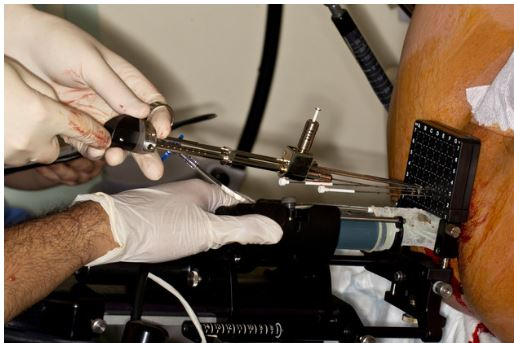
\includegraphics[width=0.5\textwidth]{Imagens/aplicadorMick.JPG}
						}%
						\caption{Aplicador MICK utilizado na Braquiterapia de próstata. São utilizadas agulhas para inserção das fontes.}
						\label{img:aplicadorMick}
					\end{figure}
				
				\item Os aplicadores permitem que a fonte permaneça em uma posição fixa durante todo o tratamento. \textit{\textcolor{CarnationPink}{Exemplo:}} \textit{Sonda e ovóides,    \ref{img:aplicadorSondaEOvoides}.}
				
					\begin{itemize}[label=\textcolor{CarnationPink}{$\star$}]
						\item \textcolor{DarkTurquoise}{\textbf{Sonda e ovóides:}} Esse é um tipo de aplicador utilizado na braquiterapia ginecológica, especificamente para tratamentos em vagina e útero. Consiste em uma sonda e ovóides que são inseridos no canal vaginal e na cavidade uterina, respectivamente. Esses aplicadores mantêm a fonte de radiação em uma posição fixa durante todo o tratamento, permitindo uma distribuição precisa da dose de radiação no tecido alvo.
					\end{itemize}
					\begin{figure}[h]
						\centering
						\fcolorbox{DarkTurquoise}{white}{%
							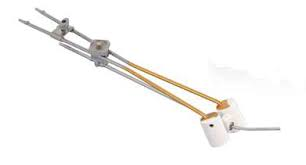
\includegraphics[width=0.5\textwidth]{Imagens/aplicadorSondaEOvoides.jpg}
						}%
						\caption{Aplicador ginecológico com sonda e ovóides.}
						\label{img:aplicadorSondaEOvoides}
					\end{figure}
			\end{enumerate}
				

			Os tipos de carregamento, por sua vez, referem-se à forma como as fontes de radiação são inseridas nos aplicadores e ao tempo que permanecem em cada posição de parada. Esse carregamento pode ser realizado de diferentes maneiras, dependendo do objetivo do tratamento e das características do tumor. Por exemplo, as fontes de radiação podem ser carregadas manualmente nos aplicadores, posicionando-as em posições pré-determinadas e mantendo-as lá por um determinado período de tempo. Essas posições de parada são estrategicamente escolhidas para garantir uma distribuição adequada da dose no tecido alvo e minimizar a dose nos tecidos saudáveis circundantes.

			O carregamento das fontes de radiação na braquiterapia pode ser classificado em diferentes métodos de acordo com a forma como as fontes são inseridas nos aplicadores. Esses métodos são:

			\begin{itemize}
				\item \textcolor{DarkTurquoise}{\textbf{Braquiterapia com pré-carregamento manual (\textit{preloaded}):}} Nesse método, as fontes de radiação são manualmente pré-carregadas nos aplicadores antes de serem inseridos no paciente. As fontes são posicionadas nas posições pré-determinadas dentro do aplicador e, em seguida, o aplicador é colocado no local desejado no tecido-alvo. Esse método é comumente utilizado em procedimentos de braquiterapia de baixa taxa de dose (LDR).
				
				\item \textcolor{DarkTurquoise}{\textbf{Braquiterapia com pós-carregamento manual (\textit{Manually afterloaded}):}} Nesse método, os aplicadores são inseridos no paciente e, em seguida, o médico realiza a inserção manual das fontes de radiação nos aplicadores. As fontes são posicionadas nas posições pré-determinadas de acordo com o plano de tratamento.
				
				\item \textcolor{DarkTurquoise}{\textbf{Braquiterapia com pós-carregamento remoto (\textit{Remotely afterloaded}):}} esse método, o aplicador é inserido no paciente e um equipamento, chamado de robô ou sistema de afterloading remoto, é utilizado para mover as fontes de radiação dentro do aplicador de acordo com as posições pré-definidas. Esse sistema permite um controle preciso e automatizado do posicionamento das fontes de radiação, garantindo a exatidão e a segurança do tratamento. Esse método é frequentemente utilizado em procedimentos de braquiterapia de alta taxa de dose (HDR), onde a capacidade de controlar com precisão a dose e a distribuição espacial da radiação é essencial.
			\end{itemize}

			O carregamento das fontes de radiação na braquiterapia também pode ser definido de acordo com a distribuição dos tempos de parada das fontes. Essa distribuição de tempos de parada afeta diretamente a distribuição de dose ao longo do aplicador. Existem dois tipos principais de carregamento nesse contexto:
		
			\begin{itemize}
				\item \textcolor{DarkTurquoise}{\textbf{Carregamento Uniforme:}} Nesse tipo de carregamento, todas as fontes de radiação com a mesma atividade permanecem o mesmo período de tempo em cada posição de parada. Isso resulta em uma distribuição de dose mais "quente"  no centro do aplicador e mais "fria" nas extremidades. Na imagem ilustrativa (\subref{fig:carregamentoUniforme}), podemos observar que a dose é mais alta no centro do aplicador e diminui gradualmente em direção às extremidades.
				

				\item \textcolor{DarkTurquoise}{\textbf{Carregamento Não-Uniforme:}} Nesse tipo de carregamento, as fontes permanecem tempos diferentes em cada posição de parada. Essa abordagem permite ajustar a distribuição de dose ao longo do aplicador para obter uma distribuição mais homogênea. Um exemplo comum é o carregamento periférico, em que as fontes permanecem por mais tempo nas posições próximas às extremidades do aplicador, resultando em uma dose mais uniforme ao longo do tecido-alvo. Na imagem ilustrativa (\Subref{fig:carregamentoPeriferico}), podemos observar que a dose é mais uniforme ao longo do aplicador, sem uma concentração excessiva de dose no centro.
				
			
					\begin{figure}[h]
						\centering
						\subfigure[Uniforme]{
							\fcolorbox{DarkTurquoise}{white}{%
								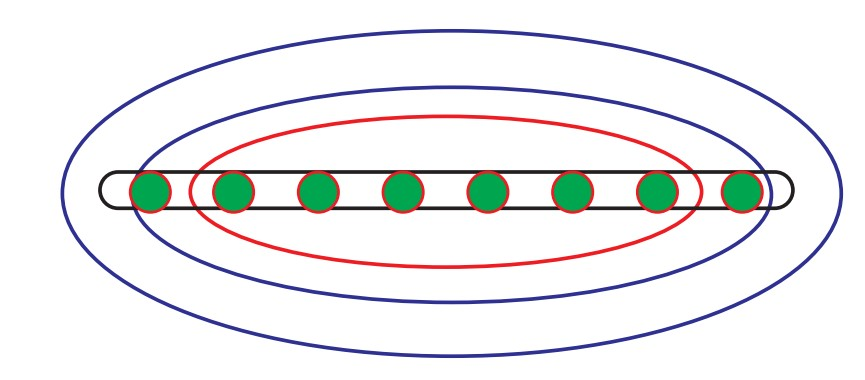
\includegraphics[width=0.4\textwidth]{Imagens/carregamentoUniforme.jpg}
								\label{fig:carregamentoUniforme}
							}}
						\subfigure[Periférico]{
							\fcolorbox{DarkTurquoise}{white}{%
								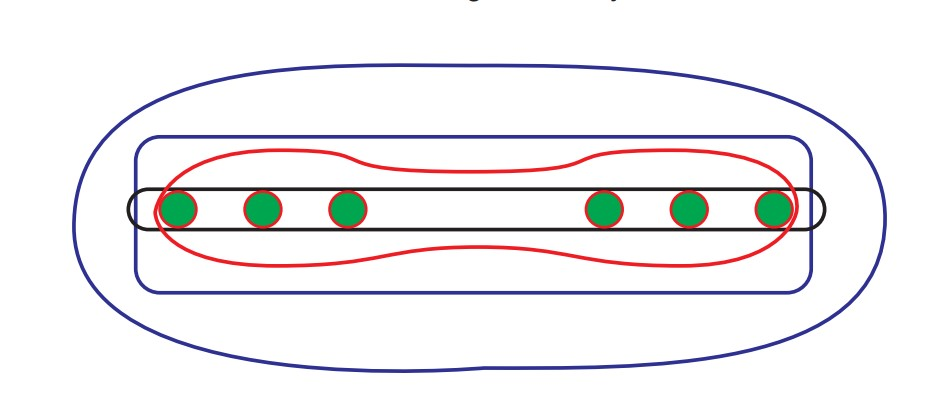
\includegraphics[width=0.4\textwidth]{Imagens/carregamentoPeriferico.jpg}
								\label{fig:carregamentoPeriferico}
							}} \\ %
						\caption{Tipos de Carregamento}
						\label{fig:tiposDeCarregamentos}
					\end{figure}
			\end{itemize}
		
	\section{Radioatividade}

		A Radioatividade é o fenômeno físico por trás das emissão de radiação pelas fontes utilizadas em braquiterapia. As principais relações físicas que caracterizam o fenômeno da Radioatividade são:

		\begin{itemize}
			\item \textcolor{DarkTurquoise}{\textbf{Desintegração por unidade de tempo:}} Mostra o número de átomos que se desintegram com o passar do tempo. 

				\begin{equation}
					\frac{dN}{dt} = -\lambda N
					\label{eq:DesintegracaoPorUnidadeDeTempo}
				\end{equation}
		
				\begin{exemplo}[onde:]
					\textcolor{CarnationPink}{$\mathbf{\frac{dN}{dt}}$} é o número de desintegrações por unidade de tempo;

					\

					\textcolor{CarnationPink}{$\mathbf{\lambda}$} é a constante de decaimento; Refere-se à taxa pela qual o número de átomos radioativos diminuem ou decaem ao longo do tempo; e

					\


					\textcolor{CarnationPink}{$\mathbf{N}$} é o número de átomos radioativos da amostra.

					\

					\textit{\textbf{\textcolor{CarnationPink}{Obs:}}} O sinal negativo na   indica que o número de átomos radioativos remanescentes na amostra diminui com o passar do tempo. 
				\end{exemplo}
				

			\item \textcolor{DarkTurquoise}{\textbf{Lei do decaimento exponencial:}} Permite obter o número de átomos radioativos em  um tempo $t$ qualquer que ainda não decaíram, ou seja, indica o número de átomos de um determinado elemento instável que não sofreram transformação.

				\begin{equation}
					N(t) = N_0 \times e^{-\lambda t}
					\label{eq:decaimentoExponencial}
				\end{equation}
				
				\begin{exemplo}[onde,]
				\begin{itemize}
					\item \textcolor{DarkTurquoise}{$\mathbf{N_0}$} é o número inicial de átomos radioativos (t = 0);
					
					\item \textcolor{DarkTurquoise}{$\mathbf{t}$} é o tempo decorrido; e

					\item \textcolor{DarkTurquoise}{$\mathbf{N(t)}$} é a quantidade de átomos radioativos remanescentes após um tempo t.
				\end{itemize}
				\end{exemplo}
				Através da   \ref{eq:decaimentoExponencial} podemos extrair que a fração de átomos que permanecem na amostra após um tempo t é dada por:

				\begin{equation}
					\frac{N(t)}{N_0}
				\end{equation}

				E a fração de átomos que decaíram da amostra é dada por:

				\begin{equation}
					1 - \frac{N(t)}{N_0}
				\end{equation}

			\item \textcolor{DarkTurquoise}{\textbf{Tempo de meia-vida ($t_{1/2}$):}} É o tempo no qual o número de átomos radioativos de uma amostra demora para decair pela metade do seu valor inicial, ou seja é o tempo para que o número de átomos radioativos remanescentes na amostra fique igual a metade do seu valor inicial, 
			
				\begin{equation}
					N(t) = \frac{1}{2}N_0
				\end{equation}

				Portanto o tempo de meia-vida  ($t_{1/2}$) é dado por:

				\begin{equation}
					t_{1/2} = \frac{\ln 2}{\lambda}
				\end{equation}

				\textbf{\textcolor{CarnationPink}{Obs:} } Podemos notar que um material radioativo com uma vida longa está relacionado com um grande tempo de veia vida e portanto um pequeno valor para a taxa de decaimento.

				Após $n$ $t_{1/2}$ temos que:

				\begin{equation}
					N = \left({1/2}\right)^n N_0
				\end{equation}

% Deduzir o porque a vida média assume que N é igual a 1/e				
			\item \textcolor{DarkTurquoise}{\textbf{Tempo de vida-média ($\tau$):}} Se caracteriza como o tempo necessário para que todos os átomos radioativos decaiam assumindo que a taxa de decaimento se mantenha fixa em seu valor inicial.
			
				\begin{equation}
					\tau = \frac{1}{\lambda}
				\end{equation}

				\begin{equation}
					\tau = 1.44 \times t_{1/2}
				\end{equation}

				\textbf{\textcolor{CarnationPink}{Obs:}} O tempo de vida média é utilizado para calcular a dose total recebida em um implante permanente pois as fontes radioativas ficarão em todo o seu tempo de vida inseridas no paciente e a vida média descreve o tempo médio total que um material permanece radioativo.

			\item \textcolor{DarkTurquoise}{\textbf{Meia Vida Biológica ($t_{biol}$):}} É o tempo que leva para a metade da fonte ser eliminada pelo próprio corpo.
			
			\item \textcolor{DarkTurquoise}{\textbf{Meia Vida Efetiva ($t_{eff}$):}} É o tempo de meia vida que considera tanto a eliminação biológica do material quanto o seu tempo de decaimento.
			
				\begin{equation}
					\frac{1}{t_{\text{eff}}} = \frac{1}{t_{1/2}} + \frac{1}{t_{\text{biol}}}
				\end{equation}

			\item \textcolor{DarkTurquoise}{\textbf{Atividade ($A$):}} É definida como o número de desintegrações por unidade de tempo, ou seja, é a taxa de decaimento de uma fonte radioativa. 
				
				\begin{equation}
					A = -\frac{dN}{dt} = \lambda N
				\end{equation}

			\item \textcolor{DarkTurquoise}{\textbf{Atividade em função do tempo ($A(t)$):}} Uma vez conhecida a atividade $A_0$ em um tempo $t_0$ qualquer, pode-se obter a atividade da fonte em função do tempo, seja ele no passado ou futuro, através da  :
				
				\begin{equation}
					A(t) = A_0 \times e^{-\lambda t}
					\label{eq:AtividadeNoTempo}
				\end{equation}

			\item \textcolor{DarkTurquoise}{\textbf{Atividade Específica:}} É definida como a atividade de um material por unidade de massa. A atividade específica é uma medida importante na produção de fontes de braquiterapia de Alta Taxa de Dose (HDR), pois está relacionada à capacidade de fornecer uma alta taxa de dose com uma quantidade reduzida de material radioativo. Uma alta atividade específica indica que uma quantidade menor de material radioativo pode ser utilizada para produzir uma fonte de braquiterapia HDR. Isso é possível porque uma alta atividade específica significa que a fonte possui uma alta atividade em relação à sua massa. Portanto, mesmo com uma quantidade menor de material radioativo, é possível obter uma taxa de dose elevada durante o tratamento. \textit{\textcolor{MediumOrchid}{Exemplo:}  A atividade específica típica do cobalto-60 é cerca de 44 terabecquerels (TBq) por grama (ou 44 TBq/g) e a atividade específica típica do irídio-192 varia de 200 a 500 terabecquerels (TBq) por grama (ou 200-500 TBq/g).}

		\end{itemize}

\section{Especificação da Fonte}
		
	A especificação da fonte de braquiterapia pode ser feita levando em consideração diferentes parâmetros, dependendo da época e dos materiais radioativos utilizados. Alguns métodos de especificação incluem a massa de Radio-226, a massa de Rádio Equivalente e a atividade da fonte.	Uma fonte pode ser especificada com base na determinação da força da fonte \textcolor{MediumOrchid}{\textit{(Source Strength)}}. Essa grandeza sofreu variações ao longo do tempo, de acordo com o surgimento de novas fontes de radiação que substituíram o Rádio-226. 

\subsection*{Massa de Radio-226}

	Forma antiga de especificação da fonte que se baseia na quantidade de material presente na amostra. Era expressa em \textcolor{MediumOrchid}{\textit{$mg\; Ra$}} que quantificava a quantidade de radiação emitida quando a única fonte de radiação utilizada em braquiterapia era o $\mathrm{{}^{226}Ra}$.

\subsection*{Massa de Rádio Equivalente}

	Com o surgimento de diferentes materiais radioativos utilizados na braquiterapia, como o Césio-137 (\ce{^{137}Ce}), foi introduzida a massa de Rádio Equivalente. Essa medida é definida como a massa de Rádio encapsulada em 0.5 mm de Platina (\ce{Pt}) que produz a mesma taxa de exposição que a fonte de interesse na posição de calibração. Essa especificação faz a equivalência com as dontes de \ce{^{226}Ra}, permitindo comparar diferentes fontes de radiação e sua capacidade de produzir a mesma taxa de exposição.

\subsection*{Atividade}

	É uma das grandezas que pode ser utilizada para especificar a fonte. Como descrito anteriormente, a Atividade é definida como o número de núcleos se submetendo ao decaimento radioativo por unidade de tempo,   \ref{eq:AtividadeNoTempo}.

			\begin{itemize}
				\item Unidade SI: \textcolor{DarkTurquoise}{\textbf{Bq}} (Becquerel) = $1\;dps$
				\item Unidade Antiga: \textcolor{DarkTurquoise}{\textbf{Ci}} (Curie) = $3.7 \times 10^{10}\; Bq$
			\end{itemize}

			\textbf{\textbf{\textcolor{CarnationPink}{Obs:} } }Embora não ser a unidade oficial do SI, o \textbf{Ci} ainda é muito utilizado na rotina clínica. \textit{\textcolor{MediumOrchid}{Exemplo:}} \textit{O Irídio-192 utilizado em tratamentos HDR possui atividade típica entre 5 Ci e 10 Ci}

\subsection*{Atividade Aparente}

	A atividade aparente é um conceito que leva em consideração a filtragem da radiação emitida pela fonte de braquiterapia devido ao encapsulamento metálico. Todas as fontes de radiação são revestidas por um material que absorve parte da radiação emitida, como por exemplo o revestimento de platina (Pt) utilizado em muitas fontes de braquiterapia.

	A atividade aparente é definida como a atividade de uma fonte pontual hipotética, não filtrada, que teria a mesma taxa de exposição na distância de calibração da fonte de interesse. Em outras palavras, é a atividade que uma fonte não blindada teria que ter para produzir a mesma taxa de exposição que a fonte blindada na distância de calibração. É uma maneira de quantificar a eficiência de filtragem da fonte e levar em consideração o efeito da blindagem no cálculo da atividade.
	
		
\subsection*{Taxa de Exposição}

	A taxa de exposição é uma medida da taxa na qual o ar é ionizado pela radiação indiretamente ionizante, como os raios gama e raios-x. Essa grandeza é definida como a taxa de carga produzida no ar pela radiação indiretamente ionizante por unidade de massa de ar.

	Quando a radiação indiretamente ionizante interage com o ar, ela produz pares elétrons-íons devido a ionizam o ar. A taxa de exposição mede o número de pares elétron-íon- produzidos por unidade de tempo e de massa de ar.

		\textit{``É o quociente entre dQ por dm, onde dQ é o valor absoluto da carga total de íons de um dado sinal, produzidos no ar, quando todos os elétrons (negativos e positivos) liberados pelos fótons no ar, em uma massa dm, são completamente freados no ar''}
		
		

			\begin{itemize}
				\item Unidade SI: $C/Kg\cdot h$
				\item Unidade Antiga: $R / h$
			\end{itemize}

			A relação entre o Roentgen e A Unidade do SI é obtida pela seguinte relação:

			\begin{equation}
				1\;R = 2.58 \times 10^{-4}\; \frac{C}{Kg}
			\end{equation}

			\textit{\textcolor{MediumOrchid}{Obs:}  é comum determinar a força de uma fonte de radiação gama em termos da taxa de exposição medida a uma distância de calibração de 1 metro da fonte. Essa distância padrão é escolhida para garantir uma comparação consistente entre diferentes fontes.}

			A uma distância específica da fonte, a taxa de exposição (\textbf{\textit{\textcolor{MediumOrchid}{$\dot{X}$}}}) está relacionada com a Atividade de uma fonte através da constante de taxa de exposição $\Gamma$.

				\begin{equation}
					\Gamma = \frac{\dot{X}(r)}{A} \cdot r^2
				\end{equation}

				\begin{exemplo}[onde,]
					\begin{itemize}
						\item \textcolor{DarkTurquoise}{$\mathbf{r}$} é a distância entre a fonte e o ponto de análise.
					\end{itemize}
				\end{exemplo}

\subsection*{Força kerma-ar}

	A força kerma-ar é uma unidade desenvolvida pela AAPM (American Association of Physicists in Medicine) para especificar a força de uma fonte de emissores gama. Essa grandeza, representada por $S_k$, é definida como o produto da taxa de kerma-ar medida em uma distância específica, denotada por $d$, a partir do centro da fonte ao longo do seu eixo transversal, multiplicada pelo quadrado da distância. 

			\begin{itemize}
				\item \textcolor{DarkTurquoise}{\textbf{Kerma}:} quantifica a energia que foi transferida para as partículas carregadas por unidade de massa em um volume do meio;
				\item \textcolor{DarkTurquoise}{\textbf{Força kerma-ar $(S_k)$:}} É a medida da energia transferida para o ar.
			\end{itemize}

	Ao multiplicar a taxa de kerma-ar pela distância $d$ ao longo do eixo transversal da fonte e pelo quadrado dessa distância, obtemos uma medida da intensidade da radiação gama em relação à distância e à área de exposição. Isso permite uma especificação mais precisa da força da fonte, considerando tanto a taxa de kerma-ar quanto a distância da fonte ao ponto de medição.

			\begin{equation}
				S_k = \dot{K}(d) \cdot d^2
			\end{equation}

			\textbf{\textcolor{MediumOrchid}{Obs:} } $S_k$ é medido no ar livre, normalmente a 1 m de distancia do centro da fonte.

			\

			A unidade no SI para a Força kerma-ar é \textbf{\textcolor{MediumOrchid}{U}}, onde


			\begin{equation}
				U = cGy \cdot cm^2 / h = \mu Gy \cdot m^2 / h
			\end{equation}

\section{Fontes Utilizadas Em Braquiterapia}
% TODO: Inserir sobre as fontes de rutênio 106 e de Californio 252 - fontes menos utilizadas

\subsubsection*{Fontes de  Fótons de Alta Energia}
		
	\begin{tcolorbox}[width=\textwidth, colback={white}, colbacktitle={DarkTurquoise!50!white}, title={$\bigstar$ \LobsterTwo{Rádio 226} $\bigstar$}, coltitle={CarnationPink}, colframe={DarkTurquoise}, fonttitle=\rmfamily\bfseries\Large, breakable]
		
			\begin{itemize}
				\item \textcolor{DarkTurquoise}{\textbf{Aplicação Clínica:}} LDR Intracavitária e Intersticial
				\item \textcolor{DarkTurquoise}{\textbf{Sítios de tratamento mais comuns:}} Historicamente utilizada
				\item \textcolor{DarkTurquoise}{\textbf{Forma da fonte:}} Tubos e agulhas
				\item \textcolor{DarkTurquoise}{\textbf{Partícula Emitida:}} Raios-$\gamma$
				\item \textcolor{DarkTurquoise}{\textbf{Energia média:}} 830 KeV
				\item \textcolor{DarkTurquoise}{\textbf{HVL:}} 12 mm de Pb
				\item \textcolor{DarkTurquoise}{\textbf{$\mathbf{t_{1/2}}$:}} 1600 anos
				\item \textcolor{DarkTurquoise}{\textbf{\% de mudança de atividade:}} 0.04\% ao ano
			\end{itemize}
	\end{tcolorbox}
			
			\

			O \textsuperscript{226}Ra foi o primeiro elemento a ser utilizado em Braquiterapia e devido a sua energia média era utilizado em vários tratamentos Intersticiais. Devido ao decaimento do \textsuperscript{226}Ra para o gás \textsuperscript{222}Rd emitindo uma partícula $\mathrm{\alpha}$ (${}_2^4He$), ocorre um aumento da pressão dentro do encapsulamento o que leva à rachaduras no envólucro da fonte, acarretando na contaminação com um material altamente danoso.

			\
		
	\begin{tcolorbox}[width=\textwidth, colback={white}, colbacktitle={DarkTurquoise!50!white}, title={$\bigstar$ \LobsterTwo{Césio 137} $\bigstar$}, coltitle={CarnationPink}, colframe={DarkTurquoise}, fonttitle=\rmfamily\bfseries\Large, breakable]
			\begin{itemize}
				\item \textcolor{DarkTurquoise}{\textbf{Aplicação Clínica:}} LDR Intracavitária e Intersticial
				\item \textcolor{DarkTurquoise}{\textbf{Sítios de tratamento mais comuns:}} Cervix e útero
				\item \textcolor{DarkTurquoise}{\textbf{Forma da fonte:}} tubos e agulhas
				\item \textcolor{DarkTurquoise}{\textbf{Partícula Emitida:}} Raios-$\gamma$
				\item \textcolor{DarkTurquoise}{\textbf{Energia média:}} 662 KeV
				\item \textcolor{DarkTurquoise}{\textbf{HVL:}} 5.5 mm Pb
				\item \textcolor{DarkTurquoise}{\textbf{$\mathbf{t_{1/2}}$:}} 30 anos
				\item \textcolor{DarkTurquoise}{\textbf{\% de mudança de atividade:}} 2.3\% por dia
			\end{itemize}
	\end{tcolorbox}
			\

			O \textsuperscript{137}Cs foi um dos substitutos do \textsuperscript{226}Ra. Por emitir uma energia média semelhante à do \textsuperscript{226}Ra, sua penetração no tecido possuía um certo grau de similaridade com o \textsuperscript{226}Ra. O \textsuperscript{137}Cs foi gradativamente sendo substituído por fontes com alta atividade com a finalidade de tornar os tempos de tratamento cada vez menores.

			O \textsuperscript{137}Cs é utilizado em sistemas afterloading de Braquiterapia LDR e foi amplamente utilizado em implantes ginecológicos LDR.

			\

		
	\begin{tcolorbox}[width=\textwidth, colback={white}, colbacktitle={DarkTurquoise!50!white}, title={$\bigstar$ \LobsterTwo{Cobalto 60} $\bigstar$}, coltitle={CarnationPink}, colframe={DarkTurquoise}, fonttitle=\rmfamily\bfseries\Large, breakable]

			\begin{itemize}
				\item \textcolor{DarkTurquoise}{\textbf{Aplicação Clínica:}} LDR Intracavitária e Intersticial e HDR Intracavitária
				\item \textcolor{DarkTurquoise}{\textbf{Sítios de tratamento mais comuns:}} Múltiplos sítios
				\item \textcolor{DarkTurquoise}{\textbf{Forma da fonte:}} fio
				\item \textcolor{DarkTurquoise}{\textbf{Partícula Emitida:}} Raios-$\gamma$
				\item \textcolor{DarkTurquoise}{\textbf{Energia média:}} 1250 KeV
				\item \textcolor{DarkTurquoise}{\textbf{HVL:}} 11 mm de Pb
				\item \textcolor{DarkTurquoise}{\textbf{$\mathbf{t_{1/2}}$:}} 5.26 anos
				\item \textcolor{DarkTurquoise}{\textbf{\% de mudança de atividade:}} 12.3\% ao ano.
			\end{itemize}
	\end{tcolorbox}

			\

			O \textsuperscript{60}Co também foi um dos substitutos do \textsuperscript{226}Ra. Um dos maiores diferenciais é que o \textsuperscript{60}Co possui uma alta atividade específica o que permite a confecção de fontes pequenas. Quando comparado ao \textsuperscript{137}Cs, é necessário uma troca de fonte com maior frequência devido o \textsuperscript{60}Co ter um tempo de meia vida menor que a do \textsuperscript{137}Cs. Portanto, para tratamentos LDR é mais interessante a utilização do \textsuperscript{137}Cs. Porém, quando comparado ao tratamento HDR com \textsuperscript{192}Ir, o \textsuperscript{60}Co pode ser uma opção mais interessante para os locais com maior dificuldade de troca de fonte.

			\

		
	\begin{tcolorbox}[width=\textwidth, colback={white}, colbacktitle={DarkTurquoise!50!white}, title={$\bigstar$ \LobsterTwo{Irídio 192} $\bigstar$}, coltitle={CarnationPink}, colframe={DarkTurquoise}, fonttitle=\rmfamily\bfseries\Large, breakable]
			\begin{itemize}
				\item \textcolor{DarkTurquoise}{\textbf{Aplicação Clínica:}} HDR Intracavitária, Intersticial e Superficial e LDR intersticial
				\item \textcolor{DarkTurquoise}{\textbf{Sítios de tratamento mais comuns:}} Cervix, útero, sarcomas, cabeça e pescoço, prostata e mama.
				\item \textcolor{DarkTurquoise}{\textbf{Forma da fonte:}} Sementes, fios e fitas
				\item \textcolor{DarkTurquoise}{\textbf{Partícula Emitida:}} Raios-$\gamma$
				\item \textcolor{DarkTurquoise}{\textbf{Energia média:}} 380 KeV
				\item \textcolor{DarkTurquoise}{\textbf{HVL:}} 2.5 mm de Pb
				\item \textcolor{DarkTurquoise}{\textbf{$\mathbf{t_{1/2}}$:}} 73.8 dias
				\item \textcolor{DarkTurquoise}{\textbf{\% de mudança de atividade:}} 0.9\% por dia
			\end{itemize}
	\end{tcolorbox}
			\

			Possui uma energia média com menor poder de penetração mas ainda sim com força suficiente para tratamentos de implantes Intersticiais feitos com o \textsuperscript{137}Cs e o \textsuperscript{60}Co. O \textsuperscript{192}Ir possui alta atividade específica o que permite a confecção de fontes pequenas, em formato de sementes e que podem ser colocadas em fitas ou fios espaçadas entre si. O \textsuperscript{192}Ir é muito utilizado em sistemas afterloading HDR.

			\

		\begin{tcolorbox}[width=\textwidth, colback={white}, colbacktitle={DarkTurquoise!50!white}, title={$\bigstar$ \LobsterTwo{Ouro 198} $\bigstar$}, coltitle={CarnationPink}, colframe={DarkTurquoise}, fonttitle=\rmfamily\bfseries\Large, breakable]
			\begin{itemize}
				\item \textcolor{DarkTurquoise}{\textbf{Aplicação Clínica:}} LDR intersticial
				\item \textcolor{DarkTurquoise}{\textbf{Sítios de tratamento mais comuns:}} Próstata
				\item \textcolor{DarkTurquoise}{\textbf{Forma da fonte:}} Sementes
				\item \textcolor{DarkTurquoise}{\textbf{Partícula Emitida:}} Raios-$\gamma$
				\item \textcolor{DarkTurquoise}{\textbf{Energia média:}} 412 KeV
				\item \textcolor{DarkTurquoise}{\textbf{HVL:}} 2.5 mm de Pb
				\item \textcolor{DarkTurquoise}{\textbf{$\mathbf{t_{1/2}}$:}} 2.7 dias
				\item \textcolor{DarkTurquoise}{\textbf{\% de mudança de atividade:}} 22.6\% por dia
			\end{itemize}
		\end{tcolorbox}
			\

			O \textsuperscript{198}Au é utilizado em forma de semente para implantes Intersticiais permanentes. Possui como vantagem uma menor energia quando comparado com o \textsuperscript{137}Cs e o \textsuperscript{60}Co. A sua meia vida curta permite ser utilizado em implantes permanentes. Sua utilização foi diminuída com a introdução do \textsuperscript{125}I

			\

\subsubsection*{Fontes de  Fótons de Baixa Energia}


		\begin{tcolorbox}[width=\textwidth, colback={white}, colbacktitle={DarkTurquoise!50!white}, title={$\bigstar$ \LobsterTwo{Iodo 125} $\bigstar$}, coltitle={CarnationPink}, colframe={DarkTurquoise}, fonttitle=\rmfamily\bfseries\Large, breakable]	
			\begin{itemize}
				\item \textcolor{DarkTurquoise}{\textbf{Aplicação Clínica:}} LDR Intersticial e Superficial
				\item \textcolor{DarkTurquoise}{\textbf{Sítios de tratamento mais comuns:}} Próstata e olho
				\item \textcolor{DarkTurquoise}{\textbf{Forma da fonte:}} sementes
				\item \textcolor{DarkTurquoise}{\textbf{Partícula Emitida:}} Raios-X
				\item \textcolor{DarkTurquoise}{\textbf{Energia média:}} 28 KeV
				\item \textcolor{DarkTurquoise}{\textbf{HVL:}} 0.025 mm de Pb
				\item \textcolor{DarkTurquoise}{\textbf{$\mathbf{t_{1/2}}$:}} 59.4 dias
				\item \textcolor{DarkTurquoise}{\textbf{\% de mudança de atividade:}} 1.2\% por dia
			\end{itemize}
		\end{tcolorbox}
			\

			É uma fonte de baixa energia amplamente utilizada no implante permanente de próstata na forma de pequenas sementes embora também possa ser utilizadas em placas oftalmológicas e em implantes cerebrais. Esta energia apresenta um acentuado falloff de dose no tecido e requer blindagem mínima para fins de radioproteção. Porém, devido a baixa dose dos fótons emitidos por esta fonte, possui uma dosimetria mais complexa e é fortemente dependente do design da fonte.

			\


		\begin{tcolorbox}[width=\textwidth, colback={white}, colbacktitle={DarkTurquoise!50!white}, title={$\bigstar$ \LobsterTwo{Paládio 103} $\bigstar$}, coltitle={CarnationPink}, colframe={DarkTurquoise}, fonttitle=\rmfamily\bfseries\Large, breakable]	
			\begin{itemize}
				\item \textcolor{DarkTurquoise}{\textbf{Aplicação Clínica:}} LDR Intersticial
				\item \textcolor{DarkTurquoise}{\textbf{Sítios de tratamento mais comuns:}} Próstata
				\item \textcolor{DarkTurquoise}{\textbf{Forma da fonte:}} Sementes
				\item \textcolor{DarkTurquoise}{\textbf{Partícula Emitida:}} Raios-x
				\item \textcolor{DarkTurquoise}{\textbf{Energia média:}} 21 KeV
				\item \textcolor{DarkTurquoise}{\textbf{HVL:}} 0.008 mm de Pb
				\item \textcolor{DarkTurquoise}{\textbf{$\mathbf{t_{1/2}}$:}} 17 dias
				\item \textcolor{DarkTurquoise}{\textbf{\% de mudança de atividade:}} 4.0\% por dia
			\end{itemize}
		\end{tcolorbox}
			\

			O \textsuperscript{103}Pd é uma alternativa ao \textsuperscript{125}I pois os fótons emitidos possuem uma energia similar porém um tempo de meia vida mais curto. O fato da meia vida o \textsuperscript{103}Pd ser mais curta fornece uma vantagem biológica pois a dose será entregue em um menor intervalo de tempo. O \textsuperscript{103}Pd é utilizado em implantes permanentes de próstata e em placas oftalmológicas.

			\

		
		\begin{tcolorbox}[width=\textwidth, colback={white}, colbacktitle={DarkTurquoise!50!white}, title={$\bigstar$ \LobsterTwo{Césio 131} $\bigstar$}, coltitle={CarnationPink}, colframe={DarkTurquoise}, fonttitle=\rmfamily\bfseries\Large, breakable]	
			\begin{itemize}
				\item \textcolor{DarkTurquoise}{\textbf{Aplicação Clínica:}} LDR Intersticial
				\item \textcolor{DarkTurquoise}{\textbf{Sítios de tratamento mais comuns:}} Próstata
				\item \textcolor{DarkTurquoise}{\textbf{Forma da fonte:}} Sementes
				\item \textcolor{DarkTurquoise}{\textbf{Partícula Emitida:}} Raios-$\gamma$
				\item \textcolor{DarkTurquoise}{\textbf{Energia média:}} 29 KeV
				\item \textcolor{DarkTurquoise}{\textbf{HVL:}} 0.025 mm de Pb
				\item \textcolor{DarkTurquoise}{\textbf{$\mathbf{t_{1/2}}$:}} 9.7 dias
				\item \textcolor{DarkTurquoise}{\textbf{\% de mudança de atividade:}} 6.9\% por dia
			\end{itemize}
		\end{tcolorbox}
			\

			o \textsuperscript{131}Cs também é uma alternativa ao \textsuperscript{125}I com uma meia vida menor e energia similar, o que também permite que a dose seja entregue em um menor intervalo de tempo.

			\

\subsubsection*{Emissores de Partículas Beta}

		\begin{tcolorbox}[width=\textwidth, colback={white}, colbacktitle={DarkTurquoise!50!white}, title={$\bigstar$ \LobsterTwo{Fósforo 32} $\bigstar$}, coltitle={CarnationPink}, colframe={DarkTurquoise}, fonttitle=\rmfamily\bfseries\Large, breakable]	
			\begin{itemize}
				\item \textcolor{DarkTurquoise}{\textbf{Aplicação Clínica:}} LDR Superficial
				\item \textcolor{DarkTurquoise}{\textbf{Sítios de tratamento mais comuns:}} pele
				\item \textcolor{DarkTurquoise}{\textbf{Forma da fonte:}} discos, placas ou fios
				\item \textcolor{DarkTurquoise}{\textbf{Partícula Emitida:}} partícula-$\beta$
				\item \textcolor{DarkTurquoise}{\textbf{Energia média:}} 695 KeV
				\item \textcolor{DarkTurquoise}{\textbf{Energia máxima:}} 1710 KeV
				\item \textcolor{DarkTurquoise}{\textbf{HVL:}} N/A
				\item \textcolor{DarkTurquoise}{\textbf{$\mathbf{t_{1/2}}$:}} 14.3 dias
			\end{itemize}
		\end{tcolorbox}

			\

			O \textsuperscript{32}P é um \textit{\textcolor{CarnationPink}{emissor beta puro}} que pode ser utilizado em um disco ou em placas para o tratamento de lesões na pele. Pode também ser utilizado em fios para o tratamento de braquiterapia vascular intervencionista de restenose in-stent de artéria cardíaca.

			\

		\begin{tcolorbox}[width=\textwidth, colback={white}, colbacktitle={DarkTurquoise!50!white}, title={$\bigstar$ \LobsterTwo{Estrôncio 90} $\bigstar$}, coltitle={CarnationPink}, colframe={DarkTurquoise}, fonttitle=\rmfamily\bfseries\Large, breakable]
			\begin{itemize}
				\item \textcolor{DarkTurquoise}{\textbf{Aplicação Clínica:}} LDR Superficial
				\item \textcolor{DarkTurquoise}{\textbf{Sítios de tratamento mais comuns:}} Olhos
				\item \textcolor{DarkTurquoise}{\textbf{Forma da fonte:}} Sementes, placas ou aplicadores
				\item \textcolor{DarkTurquoise}{\textbf{Partícula Emitida:}} partícula-$\beta$
				\item \textcolor{DarkTurquoise}{\textbf{Energia média:}} 196 KeV 
				\item \textcolor{DarkTurquoise}{\textbf{Energia máxima:}} 546 KeV
				\item \textcolor{DarkTurquoise}{\textbf{HVL:}} N/A
				\item \textcolor{DarkTurquoise}{\textbf{$\mathbf{t_{1/2}}$:}} 28.9 anos
				\item \textcolor{DarkTurquoise}{\textbf{\% de mudança de atividade:}} 2.4\% por dia
			\end{itemize}
		\end{tcolorbox}

		\begin{tcolorbox}[width=\textwidth, colback={white}, colbacktitle={DarkTurquoise!50!white}, title={$\bigstar$ \LobsterTwo{Ítrio 90} $\bigstar$}, coltitle={CarnationPink}, colframe={DarkTurquoise}, fonttitle=\rmfamily\bfseries\Large, breakable]
			\begin{itemize}
				\item \textcolor{DarkTurquoise}{\textbf{Aplicação Clínica:}} LDR Superficial
				\item \textcolor{DarkTurquoise}{\textbf{Sítios de tratamento mais comuns:}} Olhos
				\item \textcolor{DarkTurquoise}{\textbf{Forma da fonte:}} placas ou micro-esferas
				\item \textcolor{DarkTurquoise}{\textbf{Partícula Emitida:}} partícula-$\beta$
				\item \textcolor{DarkTurquoise}{\textbf{Energia média:}} 933 KeV 
				\item \textcolor{DarkTurquoise}{\textbf{Energia máxima:}} 2280 KeV
				\item \textcolor{DarkTurquoise}{\textbf{HVL:}} N/A
				\item \textcolor{DarkTurquoise}{\textbf{$\mathbf{t_{1/2}}$:}} 64.1 h 
			\end{itemize}
		\end{tcolorbox}

		\

			O \textsuperscript{90}Y é um \textit{\textcolor{MediumOrchid}{emissor beta puro}} e tanto o \textsuperscript{90}Sr como o \textsuperscript{90}Y são utilizados em placas oftalmológicas ou em tratamentos de alguns tipos de canceres em regiões que não pode haver uma profundidade de penetração da radiação no tecido. Além disso, o \textsubscript{90}Y é utilizado em micro-esferas para o tratamento de doenças hepáticas, onde as micro-esferas são produzidas com vidro ou resina incorporando o nuclídio.

		\

\section{Distribuição de Dose em Braquiterapia}

\begin{wrapfigure}{l}{0.4\textwidth}
	\centering
	\fcolorbox{DarkTurquoise}{white}{%
	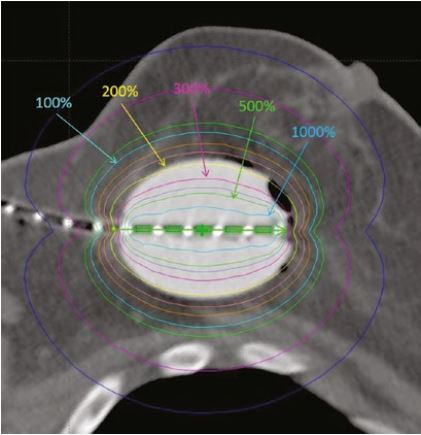
\includegraphics[width=0.35\textwidth]{Imagens/falloffDoseMammosite.JPG}
	}%
	\caption{Distribuição de dose com um balão de mama inflado.}
	\label{img:DistribuicaoDoseBalao}
\end{wrapfigure}

	A distribuição de dose em braquiterapia é caracterizada por um alto gradiente de dose e um falloff de dose mais rápido em comparação à teleterapia. Isso ocorre devido à baixa energia dos fótons emitidos pelas fontes de braquiterapia, que geralmente estão na faixa de kiloeletronvolts (KeV).


	Esse alto gradiente de dose é uma vantagem importante, pois permite uma maior preservação dos tecidos saudáveis adjacentes ao alvo. No entanto, essa mesma característica pode tornar desafiador alcançar uma distribuição de dose adequada no alvo quando este está distante da fonte, uma vez que aumentar a dose no alvo também resultaria em um aumento da dose nos tecidos próximos. Para minimizar a dose nos tecidos circundantes, recomenda-se o uso do maior aplicador possível, a fim de afastar esses tecidos da fonte e expô-los a um gradiente de dose menor em uma região mais distante.
	

	
	A precisão no posicionamento da fonte de braquiterapia é de extrema importância, uma vez que pequenas discrepâncias de milímetros podem ter um impacto significativo no tratamento. Isso ocorre devido à forma do falloff de dose, que é bastante acentuado em braquiterapia. Portanto, é necessário um posicionamento preciso da fonte, especialmente em sistemas de afterloading remoto, onde a fonte é inserida e removida do aplicador através do robô. O uso de técnicas avançadas, como a imagem por ressonância magnética (MRI) em tempo real, pode auxiliar no posicionamento preciso da fonte em relação ao alvo.
	
	A Figura \ref{img:DistribuicaoDoseBalao} ilustra as isodoses próximas à fonte e na profundidade de prescrição em um tratamento de mama utilizando um balão. A dose de prescrição está a 1 cm de profundidade da superfície do balão. Caso o balão seja esvaziado, a dose nesse mesmo ponto pode ficar 10 vezes maior que a dose de prescrição. É possível observar o falloff acentuado da dose em relação à distância da fonte, o que permite uma dose mais alta no alvo e uma dose reduzida nos tecidos circundantes.

		Existem três fatores principais que impactam a forma da distribuição de dose em braquiterapia:  \textit{\textcolor{MediumOrchid}{distância da fonte, forma e encapsulamento e o material do encapsulamento}}.

		\begin{enumerate}
			\item \textcolor{DarkTurquoise}{\textbf{A distância da fonte é um fator crucial na distribuição de dose.}} Para distâncias grandes em relação à fonte, geralmente duas vezes ou mais o tamanho da fonte, a distribuição de dose é governada pela "lei do inverso quadrado". Essa lei estabelece que a dose diminui proporcionalmente ao quadrado da distância da fonte. No entanto, à medida que o ponto de análise se aproxima da fonte, a aplicabilidade da lei do inverso quadrado diminui e outros efeitos da distância passam a ser considerados.
			
			\item \textcolor{DarkTurquoise}{\textbf{A forma cilíndrica da fonte influencia a distribuição de dose ao longo de seu eixo longitudinal.}} Devido à geometria cilíndrica, a dose ao longo desse eixo é reduzida em comparação ao eixo axial. Isso ocorre porque a radiação precisa penetrar em uma maior quantidade de material ao longo do eixo longitudinal, resultando em uma maior filtragem da radiação nessa direção. A Figura \ref{img:distribuicaoDeDose} ilustra o comportamento da distribuição de dose ao longo do eixo longitudinal da fonte.
			
				\begin{figure}[h]
					\centering
					\fcolorbox{DarkTurquoise}{white}{%
					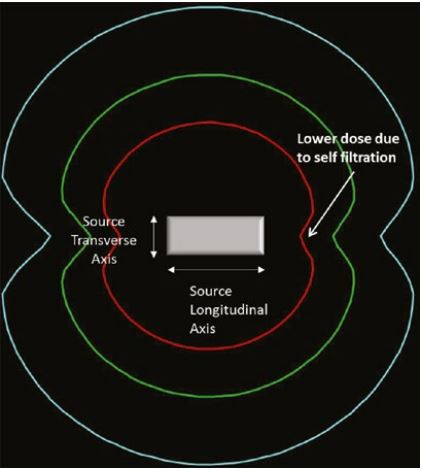
\includegraphics[width=0.4\textwidth]{Imagens/distribuicaoDeDose.JPG}
					}%
					\caption{Distribuição de dose na água para uma fonte realística de $\mathrm{{}^{192}Ir}$}
					\label{img:distribuicaoDeDose}
				\end{figure}

			\item \textcolor{DarkTurquoise}{\textbf{O material do encapsulamento da fonte também desempenha um papel importante na distribuição de dose.}} O material do encapsulamento está diretamente relacionado à absorção e ao espalhamento dos fótons emitidos pela fonte. Esses processos causam uma atenuação da radiação, afetando a forma e a intensidade da distribuição de dose.
		\end{enumerate}
	
\section{Métodos de Cálculo de Dose}

		Existem diferentes métodos para obtenção da Dose envolvida em procedimentos de braquiterapia. 

\subsection*{Cálculos de Dose Cumulativa}

	São utilizados para determinar a dose total entregue ao longo de todo o período de tratamento. Como a atividade muda com o decorrer do tempo, a taxa de dose também muda com o decorrer do tempo e pode ser obtida através da seguinte relação:

				\begin{equation}
					\dot{D}(t) = \dot{D_0} e^{-\lambda t}
					\label{eq:taxaDeDose}
				\end{equation}

	\begin{exemplo}[onde,]
		\begin{itemize}
			\item \textcolor{DarkTurquoise}{$\mathbf{\dot{D_0}}$} é a taxa de dose inicial da amostra.
		\end{itemize}
	\end{exemplo}


	A dose total acumulada em um tempo específico pode ser obtida integrando a   \ref{eq:taxaDeDose} no tempo t, ou seja:

				\begin{equation}
					D(t) = \int_{t_0}^{t} \dot{D_0} e^{-\lambda t}\,dt
					\label{eq:integralDaDose}
				\end{equation}

	Resolvendo a integral apresentada na   \ref{eq:integralDaDose}, obtemos a relação que nos fornece a dose acumulada após um tempo t (dose total).

				\begin{equation}
					D(t) = \frac{1}{\lambda} \; \dot{D_0} \; (1 - e^{-\lambda t})
					\label{eq:doseCumulativa}
				\end{equation}

	Sabendo que $$\frac{1}{\lambda} = \tau = 1.44 t_{1/2}$$ A   \ref{eq:doseCumulativa} pode ser escrita da forma:

				\begin{equation}
					D(t) = 1.44\,t_{1/2} \,\dot{D_0} (1 - e^{-\lambda t})
				\end{equation}

\subsubsection*{Aproximação para $t >> t_{1/2}$}

	No caso de implantes permanentes cuja meia vida do elemento é curta, o tempo de tratamento será muito maior que o tempo de meia vida deste elemento pois a dose será entregue ao longo de toda a vida da fonte. Podemos fazer então uma aproximação na   \ref{eq:doseCumulativa} quando $t >> t_{1/2}$: 

	Como $$t >> t_{1/2}$$ então $$\frac{t}{t_{1/2}} >> 1$$

	Como $$\lambda = \frac{ln 2}{t_{1/2}}$$ Substituindo este valor na   \ref{eq:doseCumulativa} temos que: 

	$$ D(t) = \frac{1}{\lambda}  \; \dot{D_0} \; \left(1 - e^{-\frac{ln 2}{t_{1/2}} t}\right) $$

	$$D(t) = \frac{1}{\lambda}  \; \dot{D_0} \; \left(1 - \frac{1}{e^{ln 2 \frac{t}{t_{1/2}}}}\right)$$

	Avaliando no limite quando $\frac{t}{t_{1/2}} \rightarrow \infty$ temos:

	$$ \lim_{{\frac{t}{t_{1/2}}} \to \infty} D(t) = \lim_{{\frac{t}{t_{1/2}}} \to \infty} \frac{1}{\lambda}  \; \dot{D_0} \; \left(1 - \frac{1}{e^{ln 2 \frac{t}{t_{1/2}}}}\right)$$

	Aplicando as propriedades de limite temos

	$$\lim_{{\frac{t}{t_{1/2}}} \to \infty} D(t) = \frac{1}{\lambda} \; \dot{D_0} \;  \left(\lim_{{\frac{t}{t_{1/2}}} \to \infty} 1 - \lim_{{\frac{t}{t_{1/2}}} \to \infty} \frac{1}{e^{ln 2 \frac{t}{t_{1/2}}}}\right)$$

	Como $1/ \lambda$ e $\dot{D_0}$ são constantes e:

	$$\lim_{{\frac{t}{t_{1/2}}} \to \infty} 1 = 1$$

	$$\lim_{{\frac{t}{t_{1/2}}} \to \infty} \frac{1}{e^{ln 2 \frac{t}{t_{1/2}}}} = \frac{1}{e^{\infty}} = 0 $$

	Chegamos na equação de dose total quando $t >> t_{1/2}$:

			\begin{equation}
				D = \frac{1}{\lambda} \; \dot{D_0} = \tau \; \dot{D_0} = 1.44 \; t_{1/2} \; \dot{D_0}
				\label{eq:aproximacaoImplantesPermanentes}
			\end{equation}

\subsubsection*{Aproximação para $t << t_{1/2}$}

	Outro caso a ser avaliado, são em implantes temporários cujo tempo de exposição é muito menor que o tempo de meia vida da fonte radioativa. Podemos fazer então uma aproximação da dose total para os casos em que $t << t_{1/2}$. 


	Como $t << t_{1/2}$, então

	$$\frac{t}{t_{1/2}} << 0 $$

	Podemos então utilizar a série de taylor para expandir o termo da exponencial. 

	Para $x << 0$

	$$e^x = 1 + x + \frac{x^2}{2!} + \frac{x^3}{3!} + \dots$$

	Truncando a série na primeira ordem, pois os termos quadráticos são ínfimos, temos que

	$$ e^{-ln 2 \frac{t}{t_{1/2}}} = 1 - ln 2 \; \frac{t}{t_{1/2}}$$

	Substituindo na   \ref{eq:doseCumulativa} temos então

	$$D(t) = \frac{1}{\lambda} \; \dot{D_0} \; \left[1 - \left(1 - \ln 2 \; \frac{t}{t_1/2}\right)\right]$$

	Fazendo as devidas simplificações, chegamos na   para a dose total quando $t << t_{1/2}$

			\begin{equation}
				D(t) = \dot{D_0} \; t
				\label{eq:AproximacaoImplantesTemporarios}
			\end{equation}

	Portanto a Dose total é dada pela multiplicação da taxa de dose inicial pelo o tempo de tratamento, o que faz sentido pois a atividade de uma fonte com o tempo de meia-vida muito maior que o tempo de tratamento, não sofrerá mudanças significativas nesse curto espaço de tempo.


	Nos casos em que o tempo de tratamento é da ordem do tempo de meia vida da fonte, haverá uma mudança significativa da Atividade durante o tempo de tratamento, então a dose total é obtida através da   \ref{eq:doseCumulativa}.

\subsection*{Método de Integral e Interpolação}

	Foram métodos historicamente utilizados para os cálculos de dose em fontes com formatos tubulares ou na forma de sementes.

	O método \textbf{\textcolor{MediumOrchid}{Integral de Sievert}} subdivide a fonte em n partes iguais. As partes são divididas em partes pequenas o suficiente de forma que possam ser aproximadas para fontes pontuais. Para um determinado ponto próximo à fonte, a dose é determinada somando às contribuições das n partes considerando os fatores de correção aplicados separadamente para cada parte. Os fatores de correção utilizados são: \textit{fator distância, filtração oblíqua, atenuação e espalhamento}.

	O \textbf{\textcolor{MediumOrchid}{Método de Interpolação}} utiliza tabelas de dados de conjuntos de pontos que foram previamente obtidos através de técnicas experimentais ou de modelos teóricos. As tabelas \textit{\textcolor{MediumOrchid}{along-and-away}} foram muito utilizadas para tratamentos com $\mathrm{{}^{137}Cs}$ e dados tabelados também foram muito utilizados nos sistemas Paterson-Parker e Quimbly.

\subsection*{Formalismo Modular: TG-43}

		O formalismo TG-43 é um método padrão amplamente utilizado para calcular a taxa de dose em braquiterapia. Esse método é baseado em um modelo matemático que considera uma fonte cilíndrica simétrica e leva em conta as diferenças na distribuição de dose causadas pela forma da fonte. No entanto, é importante destacar que esse formalismo assume um meio homogêneo de água e não considera a presença de heterogeneidades em um meio não homogêneo.
		
		O formalismo TG-43 utiliza dados tabelados que foram obtidos por meio de medidas experimentais e simulações de Monte Carlo para fontes de braquiterapia conhecidas. Esses dados são utilizados nos sistemas de planejamento para calcular a distribuição de dose em diferentes pontos em relação à fonte.É importante ressaltar que o formalismo TG-43 fornece uma estimativa razoável da distribuição de dose, considerando a simetria cilíndrica da fonte. No entanto, para uma precisão ainda maior, especialmente em casos com heterogeneidades ou geometrias complexas, são necessários métodos mais avançados, como simulações de Monte Carlo e técnicas de dosimetria tridimensional.

		O TG-43 é dividido em módulos, onde cada parâmetro depende da posição do ponto de cálculo de dose em relação à fonte. A Figura \ref{img:FormalismoTg43} ilustra a geometria utilizada para o cálculo da distribuição de dose. A posição do ponto de cálculo é representada em coordenadas polares, com a distância radial $r$ do ponto até o centro da fonte e o ângulo $\theta$ formado com o eixo longitudinal da fonte (eixo z na figura), medido a partir do centro da fonte. A posição de referência para os cálculos é denominada $\mathrm{P_0(r_0, \theta_0)}$ e está localizada a 1 cm da fonte ao longo do eixo central da fonte (eixo y na figura), fazendo um ângulo $\theta_0 = \pi / 2$ com o eixo longitudinal.


				\begin{figure}[h]
					\centering
					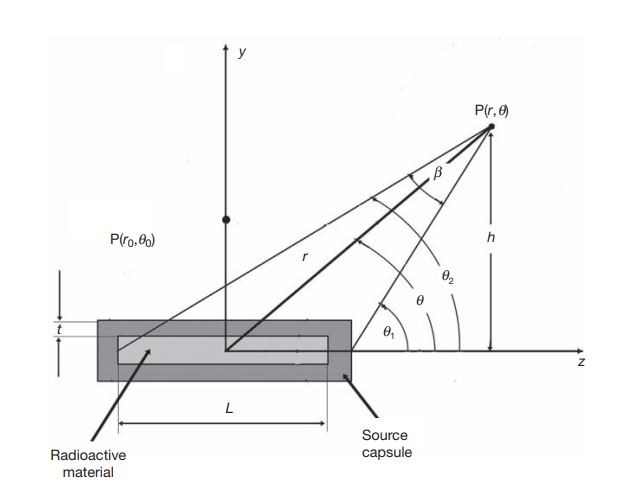
\includegraphics[width=0.8\textwidth]{Imagens/esquemaFormalismoTg43.JPG}
					\caption{Geometria Utilizada para determinação da taxa de dose no Formalismo do TG 43}
					\label{img:FormalismoTg43}
				\end{figure}

			A taxa de dose em função da posição do ponto de cálculo é dada por:

			\begin{equation}
				\dot{D}(r, \theta) = S_k \; \varLambda \; \frac{G(r, \theta)}{G(r_0, \theta_0)} 
				\; g(r) \; F(r, \theta)
				\label{eq:formalismoTg43}
			\end{equation}

			\begin{exemplo}[onde,]

			\begin{itemize}
				\item \textbf{\textcolor{DarkTurquoise}{$\varLambda$} : } é a constante de taxa de dose responsável por corrigir a medida no ar para a água. É definida como a taxa de dose na água por unidade de força Kerma-ar na posição de referência $\mathrm{P_0(r_0, \theta_0)}$. A utilização da constante $\varLambda$ permite que os cálculos de dose sejam realizados para um meio homogêneo de água, o que é mais adequado para simular a interação da radiação com o tecido do paciente. Embora a força Kerma-ar seja definida no ar, a correção por meio da constante $\varLambda$ possibilita que os resultados sejam aproximados para um meio com características semelhantes às da água.

					\begin{equation}
						\varLambda = \frac{\dot{D}(r_0, \theta_0)}{S_k}
					\end{equation}

					$$[\varLambda] = cGy / U \cdot h$$

				É importante reafirmar que, embora a utilização da constante $\varLambda$ permita uma estimativa mais precisa da distribuição de dose, o formalismo TG-43 ainda não considera as heterogeneidades presentes nos tecidos do paciente.

				\item \textbf{\textcolor{DarkTurquoise}{$S_k$} : } É a força Kerma-ar. É definida como a taxa kerma-ar medida no ar livre em uma distância específica do centro da fonte ao longo do seu eixo transversal multiplicado pelo quadrado da distância do ponto à fonte.

					\begin{equation}
						S_k = \dot{K}(d) \cdot d^2
					\end{equation}

					$$[S_k] = U = cGy \cdot cm^2 / h$$

				\item \textbf{\textcolor{DarkTurquoise}{$G(r, \theta)$}: } É a função Geométrica. 
				A função geométrica ($G(r, \theta)$) é um parâmetro utilizado levar em consideração a distribuição espacial da atividade dentro da fonte, ou seja, a forma da fonte de radiação. Ela fornece a efetiva lei do inverso quadrado ao considerar a variação da dose relativa devido à distribuição espacial da atividade. A função geométrica depende apenas da distância radial e angular do ponto de análise em relação à fonte. Ela não leva em consideração o espalhamento e a atenuação da radiação, focando exclusivamente na queda de dose com base na lei do inverso quadrado efetiva para a geometria da fonte.
				
					$$[G(r_ \theta)] = cm^{-2}$$

					Para uma fonte Pontual:

					\begin{equation}
						G(r, \theta) = \frac{1}{r_2}
					\end{equation}

					Para uma fonte cilíndrica:

					\begin{equation}
						G(r, \theta) = \frac{\beta}{L \; r \; sen(\theta)}, \qquad para \qquad \theta \neq 0
					\end{equation}

					\begin{equation}
						G(r, \theta) = \left(r^2 - \frac{L^2}{4}\right)^{-1}, \qquad para \qquad \theta = 0
					\end{equation}
				
				\item \textbf{\textcolor{DarkTurquoise}{$g(r)$} : } É chamada de Função de dose radial. Ela leva em conta o espalhamento e a atenuação da radiação no material do encapsulamento da fonte, assim como a transição do meio de ar para água.

				A função de dose radial é adimensional e é definida ao longo do eixo transversal da fonte, com o ângulo $\theta$ igual a $\pi / 2$. Portanto, ela depende apenas da distância radial do ponto de análise em relação à fonte.
				
				O espalhamento da radiação aumenta a dose na profundidade, enquanto a atenuação da radiação diminui a dose na profundidade. A função de dose radial quantifica essas alterações e reflete a distribuição de dose ao longo do plano transversal da fonte.
				
				Os valores da função de dose radial são tabelados e podem ser encontrados em publicações, como o update do TG-43 e em seu suplemento. Esses valores são determinados por meio de estudos experimentais e simulações de Monte Carlo para diferentes tipos de fontes de braquiterapia.
				
					Na distância de referência $r_0$

					$$g(r_0) = 1$$
				
				\item \textbf{\textcolor{DarkTurquoise}{$F(r, \theta)$} : } É chamada de Função de Anisotropia. A função de anisotropia, representada por $F(r, \theta)$, é uma medida que leva em consideração o formato anisotrópico da distribuição de dose causado pela própria filtração do encapsulamento da fonte e a transmissão oblíqua através do encapsulamento. Ela fornece a distribuição de dose para ângulos diferentes de $\theta = \pi / 2$, ou seja, para pontos em ângulos fora do eixo transversal da fonte.

				Em outras palavras, a função de anisotropia é responsável por quantificar a variação da dose em relação ao ângulo polar formado com o plano transversal da fonte. Isso ocorre porque a filtração e a transmissão oblíqua da radiação pelos materiais do encapsulamento afetam a distribuição de dose em diferentes direções. Portanto, a função de anisotropia nos permite entender como a dose se comporta em ângulos diferentes em relação ao eixo transversal da fonte.
				
					Para $\theta = \theta_0 = \pi/2$

					$$F(r, \theta_0) = 1$$

			\end{itemize}
		\end{exemplo}

\subsubsection*{Aproximação Para Fontes Pontuais}
			
			Ao aplicar a equação \ref{eq:formalismoTg43} para uma fonte pontual, é possível desconsiderar a anisotropia da distribuição de dose em função do ângulo. Isso ocorre porque a distribuição de dose para uma fonte pontual é isotrópica na mesma distância radial, ou seja, a dose é igual em todas as direções a partir do ponto central.

			Nesse caso, a função de anisotropia $F(r, \theta)$ pode ser substituída por um fator de anisotropia 1D, representado por $\Phi(r)$. Essa função é calculada pela média da taxa de dose em cada distância em relação ao ângulo sólido, desconsiderando a dependência angular. Dessa forma, o fator de anisotropia $\Phi(r)$ representa a média da distribuição de dose em relação à posição radial.

			Essa simplificação é válida para fontes pontuais, onde não há variação significativa da distribuição de dose em função do ângulo. A isotropia da dose em uma distância radial específica simplifica o cálculo, uma vez que a distribuição de dose passa a depender apenas da posição radial em relação à fonte.

			É importante ressaltar que essa simplificação só é aplicável para fontes pontuais, e em casos onde a anisotropia da distribuição de dose é desprezível. Para fontes com formato anisotrópico, como fontes alongadas ou em forma de agulhas, a função de anisotropia $F(r, \theta)$ deve ser considerada para uma análise precisa da distribuição de dose em diferentes ângulos em relação à fonte.
			
			\begin{equation}
				\dot{D}(r) = S_k \; \varLambda \; \left(\frac{r_0}{r} \right)^2 \; g(r) \; \Phi (r)
				\label{eq:aproxModularFontePontual}
			\end{equation}
			
			A Aproximação fornecida pela   \ref{eq:aproxModularFontePontual} pode ser aplicada sempre que:

			\begin{enumerate}
				\item A distância do ponto até a fonte é de no mínimo duas vezes o tamanho efetivo da fonte de modo que a forma da distribuição de dose nesse ponto não cause impacto no cálculo da dose.
				\item Quando as fontes estão distribuídas aleatoriamente de forma que é tomada uma média dos efeitos de anisotropia.
			\end{enumerate}

			Tratamentos de próstata com LDR são um exemplo de aproximação para fonte pontual enquanto que os tratamentos HDR utilizam o formalismo padrão para as fontes cilíndricas.  No tratamento de braquiterapia de próstata com LDR (baixa taxa de dose), a fonte utilizada geralmente é um implante permanente de sementes radioativas, como o Iodo-125 ou Paládio-103. Nesse caso, as sementes são implantadas diretamente na próstata, o que resulta em uma distribuição de dose mais isotrópica na região do alvo.

			Devido à distribuição relativamente aleatoriamente das sementes dentro da próstata, o tratamento pode ser aproximado como uma fonte pontual. Isso significa que a distribuição de dose ao redor das sementes é considerada isotrópica e depende apenas da distância radial em relação à semente. Portanto, para esses tratamentos, é possível utilizar uma função de anisotropia simplificada (\ref{eq:aproxModularFontePontual}).
			
			Já nos tratamentos de braquiterapia de alta taxa de dose (HDR), as fontes utilizadas são geralmente fios ou catéteres contendo material radioativo, como o Irídio-192. Essas fontes cilíndricas são inseridas temporariamente no paciente e possuem uma distribuição de dose mais anisotrópica devido à geometria do implante.
			
			Para esses casos, é necessário considerar o formalismo completo do TG-43 (\ref{eq:formalismoTg43}), levando em conta a função de anisotropia $F(r, \theta)$ para descrever a distribuição de dose em diferentes ângulos em relação ao eixo longitudinal da fonte. A geometria cilíndrica da fonte e o formato anisotrópico da distribuição de dose tornam necessário considerar a dependência angular para uma precisão adequada nos cálculos de dose.

			\begin{table}[!h]
				\centering
				\captionsetup{labelfont={color=MediumOrchid, bf}}
				\caption{\textcolor{MediumOrchid}{Valores dos parâmetros necessários para a resolução do exercício.}}
				\label{tb:paramExercCalcDose}
				\begin{tabular}{c c}
				\hline
				\multicolumn{2}{c}{Valores para r = 3.0 cm } \\
				\multicolumn{2}{c}{considerando uma fonte pontual} \\
				\midrule[1.5pt]
				Parâmetro & Valor \\
				\addlinespace[4pt]
				\midrule[1.5pt]
				$S_k$ & $0.5 \; U$ \\
				\addlinespace[4pt]
				\hline
				$\varLambda$ & $1.036 \; cGy  \cdot h^{-1} \cdot U^{-1}$ \\
				\addlinespace[4pt]
				\hline
				$g_p(r)$ & $0.702$ \\
				\addlinespace[4pt]
				\hline
				$\phi_{an}(r)$ & $0.951$ \\
				\addlinespace[4pt]
				\hline
				\multirow{2}{*}{$t_{1/2}$} & $59.4 \; dias$\\
				 & $1425.6 h$ \\
				\addlinespace[4pt]
				\hline
				 $r_0$ & $ 1 \; cm$ \\
				\addlinespace[4pt]
				\hline
				\hline
				
				\end{tabular}
			\end{table}
			
		\begin{exemplo}[Exemplo: Tratamento de Próstata com fontes de Baixa Energia]
		
			\textit{É comum ser realizado um planejamento intra-operatório para implantes de próstata onde é adquirida uma imagem de ultrasonografia transretal, que é transferida para o sistema de planejamento. Na imagem são delineados o volume alvo, o reto e a uretra. Normalmente o sistema de planejamento assumo os cálculos de distribuição de dose para uma fonte pontual. Modelos de fontes lineares podem ser utilizados desde que parta do pressuposto que essas fontes são paralelas às agulhas, porém essa forma pode levar à imprecisões nos cálculos de dose. Por outro lado, a orientação das fontes podem ser mais precisamente definidas utilizando uma imagem de Tomografia Computadorizada (TC) durante a avaliação da dose pós-implante através de métodos de segmentação automatizados. Nestes casos a distribuição de dose pode ser calculada através da soma da dose de cada semente.}

			\begin{enumerate}
				\item \textbf{As sementes do modelo Amersham 6702 de \textsuperscript{125}I são utilizadas em um implante de próstata. A força Kerma-ar para estas sementes é de 0.5 U. Uma semente está a 3.0 cm da parede anterior do reto.}
				
					\begin{enumerate}[label=\textcolor{CarnationPink}{(\alph*)}]
						\item \textbf{Qual é a taxa de dose dessa semente até o ponto mais próximo do reto?}
						\item \textbf{Quanta dose este ponto receberá da fonte após 1 mês?}
						\item \textbf{Qual a dose total que será recebida devido à esta fonte?}
					\end{enumerate}
			\end{enumerate}

			\textbf{\textcolor{CarnationPink}{Solução:}}

				\textit{A dose neste caso deve ser avaliada utilizando a aproximação para uma fonte pontual pois embora a dose seja calculada para apenas uma semente, o ponto de análise está a uma distância superior a 2 vezes o tamanho da fonte. De acordo com o TG-43, este modelo de fonte possui comprimento \textcolor{MediumOrchid}{L = 3.0 mm}.}

				Os valores das quantidades necessárias para determinação da dose foram obtidos no update do TG-43 e todos os dados necessários para os cálculos podem ser conferidos na Tabela \ref{tb:paramExercCalcDose}.

				\

				\textcolor{DarkTurquoise}{\textbf{(a)}} A taxa de dose  no ponto é então:

					$$\dot{D}(r) = S_k \cdot \varLambda \cdot \left(\frac{r_0}{r}\right)^2 \cdot g(r) \cdot \phi_{an}(r)$$
				
					Fazendo as devidas substituições temos:

					$$\dot{D}(r= 3cm) = 0.5 \cdot 1.036 \cdot \left(\frac{1}{3}\right)^2 \cdot 0.702 \cdot 0.951$$

					Portanto, temos que

					$$\dot{D}(r= 3cm) = 0.0384 \; cGy / h$$

				\textcolor{DarkTurquoise}{\textbf{(b)}} A dose acumulada após 1 mês de implante devido à fonte pode ser obtida através da  :

					$$D(t) = \dot{D_0} \cdot 1.44 \cdot t_{1/2} \cdot \left(1 - e^{- ln 2 \cdot \frac{t}{t_{1/2}}}\right)$$

					Sendo $t = 30 \; dias$, e utilizando a taxa de dose inicial obtida no item (a), temos então que:

					$$D(t = 30 \; dias) = 0.0384 \cdot 1.44 \cdot 1425.6 \cdot \left(1 - e^{- 0.693 \cdot \frac{30}{59.4}}\right) $$

					Portanto, a dose após 1 mês de implante é:

					$$D(t = 30 \; dias) = 23.28 \; cGy$$

				\textbf{\textcolor{MediumOrchid}{Obs:}} \textit{O valor da meia vida dentro da exponencial foi utilizado em dias para ficar da mesma dimensão do tempo de implante; Fora da exponencial foi utilizado em horas para obter a dose em Gy uma vez que a taxa de dose foi determinada em Gy/h, caso contrário essa conversão deveria ter sido feita no final do exercício.}

				\

				\textcolor{DarkTurquoise}{\textbf{(c)}} A dose total para um implante permanente cuja meia vida é muito menor que o tempo do implante é obtida através da relação:

					$$D = 1.44 \cdot \dot{D_0} \cdot t_{1/2}$$

					Portanto a dose total recebida no ponto devido a esta fonte será de:

					$$D = 1.44 \cdot 0.0384 \cdot 1425.6$$
					$$D = 78.83 \; cGy$$

				\textbf{\textcolor{MediumOrchid}{Obs:}} \textit{ A dose no ponto foi calculada para a contribuição de apenas 1 semente. Para obter a dose total recebida nesse ponto deve-se somar a contribuição de todas as fontes inseridas no implante.}



			
		\end{exemplo}


		
\subsection*{Sistemas Clássicos para Implantes Intersticiais}

			Antes da era computacional, eram utilizadas tabelas pré-calculadas para determinar a quantidade de rádio necessária em um \textit{\textbf{\textcolor{MediumOrchid}{Implante Intersticial}}}.

			\begin{figure}[h]
				\centering
				\fcolorbox{DarkTurquoise}{white}{%
				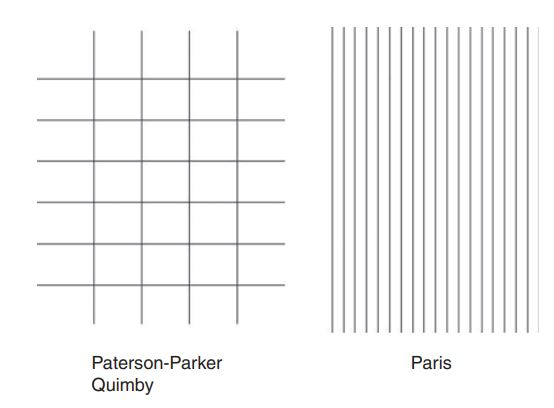
\includegraphics[width=0.7\textwidth]{Imagens/carregamentosHistoricos.JPG}}%
				\caption{Sistemas de Carregamento Clássicos}
				\label{img:carregamentosHistoricos}
			\end{figure} 


			\begin{itemize}
				\item \textcolor{DarkTurquoise}{\textbf{Sistema Manchester (Paterson-Parker)}}
				
				O Sistema Manchester, também conhecido como Sistema Paterson-Parker, é um método de braquiterapia utilizado especialmente no tratamento de câncer de colo de útero. Nesse sistema, são utilizadas agulhas ou cateteres perpendiculares entre si, formando uma estrutura chamada de "crossed ends", como mostra a \ref{img:carregamentosHistoricos}. 
				
				O sistema de dosimetria Patterson-Parker é então projetado para alcançar uma distribuição de dose uniforme dentro do volume tratado, com uma tolerância de $\pm$10\% em relação à dose prescrita ou indicada. A distribuição das fontes de radiação neste sistema segue regras específicas, principalmente com base no tamanho do volume-alvo. Normalmente, uma maior intensidade de fontes é concentrada na periferia do volume. A dose prescrita geralmente é definida em torno de 10\% acima da dose mínima dentro do volume tratado.

				As tabelas de dose Patterson-Parker fornecem valores acumulados de intensidade de fonte necessários para administrar uma dose de 900 cGy, considerando fatores atuais e unidades de dose, em função da área (para implantes planares) ou volume.

				Os princípios aplicados em diferentes cenários dentro do sistema Patterson-Parker são:

				\begin{enumerate}[label=\textcolor{CarnationPink}{(\roman*)}]
					\item \textcolor{DarkTurquoise}{\textbf{Plano Único:}} Nesse arranjo, uma camada de tecido com 1 cm de espessura é tratada, e a dose prescrita é administrada em um plano paralelo localizado a 0.5 cm de distância do plano da fonte.

					\item \textcolor{DarkTurquoise}{\textbf{Plano Duplo:}} Camadas mais espessas de tecido, normalmente de até cerca de 2.5 cm, são tratadas com fontes colocadas em dois planos paralelos. A intensidade total da fonte necessária é dividida igualmente entre os dois planos, seguindo as regras de distribuição usadas para implantes em plano único. Fatores de correção são aplicados para separações entre os planos maiores que 1 cm, para garantir que a dose mínima não seja mais do que 10\% menor do que a dose prescrita. A dose prescrita é administrada em cada plano interior, que está localizado a 0,5 cm dos planos da fonte. É importante observar que, para volumes-alvo espessos, a dose no plano médio pode ser até 20-30\% menor do que a dose prescrita.
					
					\item \textcolor{DarkTurquoise}{\textbf{Outros Volumes:}} Para diferentes formas de volumes, como cilindros, esferas ou sólidos retangulares, as regras de distribuição seguem o conceito de proporção entre casca e núcleo. Normalmente, 75\% da intensidade da fonte é colocada na casca (região periférica), enquanto 25\% é colocada no núcleo (região central).
				\end{enumerate}
				
				\item \textcolor{DarkTurquoise}{\textbf{Sistema Quimbly:}}
				
				O Sistema Quimby é outro método de braquiterapia que utiliza agulhas ou cateteres perpendiculares entre si, semelhante ao Sistema Manchester. No entanto, a principal diferença entre esses sistemas está no tipo de carregamento utilizado.

				Enquanto o Sistema Manchester emprega o carregamento não uniforme periférico para obter uma distribuição de dose homogênea ao longo do alvo, o Sistema Quimby utiliza o carregamento uniforme, resultando em uma distribuição de dose com um ponto quente central no volume implantado. Nesse sistema, as fontes de radiação são posicionadas de forma a fornecer uma dose  em todo o volume do implante, incluindo uma região central que recebe uma dose mais alta, conhecida como ponto quente.

				O sistema Quimby é baseado em uma distribuição uniforme da força da fonte, aceitando uma distribuição não uniforme da dose. Normalmente, a dose no centro do volume de tratamento é maior do que a dose próxima à periferia. O valor da dose obtido nas tabelas Quimby é a dose mínima dentro do volume implantado. Observe que, para aplicadores de superfície, a dose indicada é a dose máxima no plano de tratamento. Normalmente, para entrega de uma dose a implantes planos ou de volume de tamanho semelhante, a força total da fonte necessária ao usar o sistema Quimby será muito maior do que a exigida pelo sistema Patterson-Parker para entregar a mesma dose.
				
				\item \textcolor{DarkTurquoise}{\textbf{Sistema Paris:}}
				
				O Sistema Paris é um método de braquiterapia utilizado para implantes em planos únicos ou duplos e não aborda os outros tipos de implante de volume. Nesse sistema, são utilizadas múltiplas agulhas ou cateteres paralelos entre si, que são inseridos no tecido-alvo de forma igualmente espaçada. Uma característica importante do Sistema Paris é o carregamento uniforme das fontes de radiação. Isso significa que as fontes são colocadas de forma a fornecer uma dose não uniforme em todo o volume do implante, resultando em um ponto quente central, onde a dose é mais alta, rodeado por uma dose gradualmente decrescente.

				É necessário seguir um conjunto de regras gerais para a seleção e colocação das fontes a fim de alcançar as distribuições de dose desejadas. As regras gerais são as seguintes:

				\begin{enumerate}[label=\textcolor{CarnationPink}{(\roman*)}]
					\item As fontes devem ser lineares e sua colocação paralela;
					\item Os centros de todas as fontes devem estar localizados no mesmo plano (central
					avião)
					\item A força da fonte linear (atividade) deve ser uniforme e idêntica para todas as fontes;
					\item Fontes adjacentes devem estar equidistantes umas das outras;
					\item O espaçamento entre as fontes deve ser maior ao usar fontes longas.
				\end{enumerate}

				A taxa de dose indicada (referência) é uma porcentagem fixa (85\%) da taxa de dose basal. A taxa de dose basal é a média das taxas de dose mínima localizadas entre as fontes dentro do volume implantado. As taxas de dose mínima individual devem estar dentro de $\pm$10\% da média (taxa de dose basal), restringindo assim o número de fontes a serem usadas.

			\end{itemize}

% TODO: Sistema Classico Fletcher

\subsection*{Cálculos de Dose Baseados em Imagens}

			Algoritmos de cálculo de dose baseados em modelos podem ser utilizados para cálculos de distribuição de dose levando em consideração um meio heterogêneo, uma vez que o formalismo do TG-43 considera o meio homogêneo em seus cálculos.
			
			Os algoritmos de cálculo consideram o impacto de diferentes meios materiais na dispersão da dose através de:

				\begin{itemize}[label=\textcolor{CarnationPink}{$\blacktriangleright$}]
					\item Simulação e Acoplamento do par fóton-elétron no transporte de radiação; ou
					\item Através da utilização de técnicas de integração da dispersão multidimensional.
				\end{itemize}
			
			Os métodos de cálculos computacionais mais utilizados são:

				\begin{itemize}
					\item \textbf{\textit{\textcolor{DarkTurquoise}{Collapsed Cone Convolution-Superposition}}}, que utilizam Kernels para calcular a dose de radiação do feixe primário e do feixe espalhado no qual mapeia, espacialmente, a disposição de energia no meio. \textit{Exemplo:} \textit{\textbf{Oncentra\textsuperscript{\textregistered}}, Sistema de planejamento de braquiterapia da Elekta que implementa o algoritmo Convolution-Superposition}.
					
					\item \textbf{\textit{\textcolor{DarkTurquoise}{Grid-based Boltzmann Solvers}}}, onde é utilizada uma abordagem determinística para resolver diretamente a   de transporte linear de Boltzmann. \textit{Exemplo:} \textit{\textbf{Acuros\textsuperscript{\textregistered}}, algoritmo implementado no sistema de planejamento Brachyvision\textsuperscript{\textregistered} da Varian}.
					
					\item \textbf{\textit{\textcolor{DarkTurquoise}{Simulação de Monte Carlo}}}, que utiliza abordagens estocásticas para resolver a   de transporte linear de Boltzmann através de amostragens aleatórias. É um modelo mais presente em pesquisas científicas.
					
					\end{itemize}
		
	\section{Braquiterapia de Baixa Energia}
		

		Fontes consideradas de baixa energia são aquelas que emitem fótons com energia da ordem de 50 KeV, como o \textsuperscript{125}I, \textsuperscript{103}Pd e \textsuperscript{131}Cs.

		Devido a baixa energia dos fótons emitidos por estas fontes, a proteção radiológica se torna mais efetiva por dois motivos:

			\begin{enumerate}
				\item O feixe é atenuado pelo próprio paciente, nos casos de implantes permanentes.
				\item A blindagem de chumbo necessária para estas fontes é mínima nos casos de implantes temporários, como ocorre em placas oftalmológicas.
			\end{enumerate}
		
		As principais aplicações de fontes de braquiterapia de baixa energia são feitas nos implantes permanentes de próstata guiados por ultrassonografia transretal. Embora tenha uma aplicação mais limitada, também podem ser aplicadas no tratamento de melanomas intraoculares e tumores pulmonares em estágio inicial.

		Quando uma fonte é considerada como \textit{\textcolor{MediumOrchid}{rádio-equivalente}}, como ocorre com as fontes de \textsuperscript{137}Cs, \textsuperscript{60}Co e \textsuperscript{198}Au, seu espectro é governado por raios-$\mathrm{\gamma}$ de alta energia e podem facilmente ser especificadas em termos da definição ``\textit{miligramas de rádio equivalente}", possuindo métodos mais simples para cálculos de dose, pois a energia desses fótons é minimamente modificada pela construção da fonte e pela atenuação no tecido. 

		Porém, quando se trata de fontes de baixa energia, como o \textsuperscript{125}I, \textsuperscript{103}Pd e o \textsuperscript{131}Cs, os cálculos de dose já não são tão simples uma vez que a energia do feixe é significativamente modificada devido à atenuação e ao espalhamento dos fótons de baixa energia causados pelo encapsulamento da fonte. Para estes casos é necessária uma modificação apropriada no formalismo de cálculo para a determinação da calibração da força da fonte.

\subsection*{Design e construção das Sementes}

			O formalismo de cálculo estabelecido pelo TG-43 contemplava primordialmente os modelos de sementes:

				\begin{itemize}
					\item \textcolor{DarkTurquoise}{\textbf{\textsuperscript{125}I:}} Nycomed-Armsham 6702 e 6711
					\item \textcolor{DarkTurquoise}{\textbf{\textsuperscript{103}Pd:}} Theragenics TP-200
					\item \textcolor{DarkTurquoise}{\textbf{ \textsuperscript{192}Ir}}x: Best Medial e Alpha-Omega
				\end{itemize}
			
			O Report Tg-43 foi atualizado para corrigir inconsistências no report original e para incluir recomendações a cerca de fontes de braquiterapia de baixa energia, incluindo conjuntos de dados dosimétricos paras as novas fontes de \textsuperscript{125}I e \textsuperscript{103}Pd além dos guidelines para a determinação dos parâmetros dosimétricos das fontes de baixa energia.


			As fontes desenvolvidas possuem normalmente uma dimensão externa de 4.5 mm de comprimento e 0.8 mm de diâmetro, onde:

				\begin{itemize}
					\item O diâmetro é estabelecido sendo o mesmo diâmetro do calibre de uma agulha utilizada na braquiterapia Intersticial; E
					\item O tamanho é definido com base na regulamentação dos EUA para materiais radioativos sob a forma especial com limite de 0.5 cm para fins de embalagem e envio.
				\end{itemize}

				As características básicas de uma fonte são:

				\begin{enumerate}[label=\textcolor{CarnationPink}{(\roman*)}]
					\item Possuem um encapsulamento da fonte que deve ser feito através de uma cápsula de Titânio, sendo normalmente um tubo fino fabricado pelo processo de extrusão.
					\item Possuem envólucros de extremidades que devem ser na forma de soldas de extremidade, copos ou outros mecanismos afim de vedar os tubos de titânio após os componentes internos serem inseridos.
					\item Possuem portadores de fonte ativa que devem estar na forma de esferas ou cilindros.
					\item Possuem um material com a fonte ativa contendo o material radioativo incorporado ao portador da fonte.
				\end{enumerate}


			Em uma fonte ideal, espera-se que a distribuição de dose em volta da fonte seja uniforme e que haja uma reprodutibilidade na distribuição de dose inter-fontes. Portanto, algumas características dosimétricas podem ser afetadas devido à problemas na fabricação da fonte e portanto durante a fabricação de uma fonte deve-se atentar as seguintes características:

				\begin{itemize}[label=\textcolor{CarnationPink}{$\blacktriangleright$}]
					\item O encapsulamento da fonte deve conter uma espessura uniforme de titânio, o que é possível ser alcançado através de equipamentos de modelagem mais sofisticados.
					
					\item O projeto dos envólucros de fechamento devem ser finos e uniformes e devem garantir uma variação mínima inter-sementes. 

						\textit{Envólucros de fechamentos mais espessos, como soldas ou copos, podem aumentar a anisotropia na distribuição de dose próximo às extremidades da semente, reduzindo a precisão do cálculo da dose baseado em fontes pontuais. Variações na espessura da solda entre as sementes causam desvios nos cálculos. Essas variações, embora clinicamente insignificantes, tem o potencial de aumentar significativamente as incertezas dos valores calculados da função de anisotropia da fonte devido às incertezas nas espessuras médias das soldas de fechamento utilizada nos cálculos. Além disso, pode também aumentar a incerteza nos valores medidos de anisotropia}
					
					\item A geometria e o material dos portadores de fonte ativa podem afetar as características dosimétricas da fonte:
					
						\begin{enumerate}
							\item Utilizando \textbf{Prata} como o material do portador de fonte ativa, os raios-x da camada K desse material possuem energia de 25.51 KeV; Portanto a prata irá suavizar o espectro de energia do fotón emitido pela fonte encapsulada. Isso resulta em uma menor constante de taxa de dose em sementes de \textsuperscript{125}I com portador de prata quando comparado aos outros materiais de portadores de fonte.
							
								\textit{\textcolor{CarnationPink}{Exemplo:}} 
									\begin{itemize}
										\item Valor médio da constante de taxa de dose para o \textsuperscript{125}I encapsulado com Ag:
										
											\textbf{$\mathrm{0.953 \; cGy \cdot h^{-1} \cdot \; U^{-1}}$}
										\item Valor médio da constante de taxa de dose para outras sementes de \textsuperscript{125}I:
										
											\textbf{$\mathrm{1.026 \; cGy \cdot h^{-1} \cdot \; U^{-1}}$}
									\end{itemize}

							\item A falta de reprodutibilidade do posicionamento dos portadores da fonte dentro do encapsulamento de titânio pode afetar negativamente a precisão nas medidas da distribuição de dose em volta da fonte, semelhantemente ao que ocorre com as diferenças das espessuras da solda no fechamento da semente em sua parte interna.
							
						\end{enumerate}
					
					\item A falta de uniformidade na deposição do material da fonte radioativa nos carregadores da fonte podem aumentar os valores calculados e medidos da anisotropia da distribuição de dose e até mesmo da função de dose radial.
					
				\end{itemize}

			As incertezas na distribuição de dose devido à fabricação da fonte são reduzidas conforme tenha um aumento do número de fontes utilizadas no tratamento do paciente; Além dessa incertezas serem mais enunciadas à curtas distâncias da fonte. Pode-se afirmar então que os cálculos de dose baseados em fontes pontuais permitem precisão adequada do cálculo da dose pois são tomados à uma distância segura da fonte ou devido à contribuição de várias fontes, situações onde os erros de fabricação são desprezíveis.

			Nenhuma alteração na fabricação da fonte deve ser feita sem comunicação prévia devido a alta sensibilidade das fontes de baixa energia o que faz com que qualquer alteração pode levar a um impacto dosimétrico.

\subsection*{Dosimetria das Fontes de Baixa Energia}

			As fontes de braquiterapia são descritas com base em sua atividade aparente. A atividade aparente é obtida através da taxa de exposição na distância de calibração em um laboratório acreditado. Com bases nesses valores que foram calculados as distribuições de dose 2-D.

			O padrão para determinar a força da fonte é a \textit{\textbf{\textcolor{MediumOrchid}{Força Kerma-AR}}}, que pode ser convertida para a taxa de exposição à 1m da fonte através da relação:

				\begin{equation}
					S_k = \dot{X}(R \cdot h^{-1}) \cdot 0.876 \; (cGy/R) \cdot (1 \; m)^2
				\end{equation}
			
			A força Kerma-ar é definida como o produto da força Kerma-ar devido aos fótons de energia $\dot{K}$ maiores que a energia de corte $\delta$ a uma distância $d$ e o quadrado da distância:

				\begin{equation}
					S_k = \dot{K}_\delta (d) \cdot d^2
				\end{equation}

				\textit{\textbf{\textcolor{MediumOrchid}{Obs:}}} O valor valor para energia de corte para fótons de baixa energia é de:

				$$\delta = 5 \; \; KeV$$
				
			A força Kerma-ar em uma fonte cilíndrica pode ser calibrada através de comparação direta com uma fonte do mesmo tipo calibrada no laboratório acreditado.

			\textit{\textbf{\textcolor{MediumOrchid}{Obs:}}} O NIST é um laboratório acreditado onde a calibração é feita com uma câmara de ar livre com ampla angulação (incidência de vários ângulos) com uma aproximação de $0.01 \; \; Gy \; m^2 \; h^{-1}$. É feita uma filtragem com alumínio para excluir a contaminação com fótons de baixa energia da ordem da energia de corte na definição da Força Kerma-ar para minimizar a incerteza na medição.

			A dose 2-D é então determinada pela   \ref{eq:formalismoTg43} levando em consideração a correção feita na exposição para determinar a força kerma-ar;

		\subsection*{Aplicações Clínicas dos Fótons de Baixa Energia}

			Os raios-X de baixa energia possuem maior Transferência Linear de Energia \textbf{\textcolor{MediumOrchid}{(LET)}} quando comparados aos raios-x de alta energia. Isto resulta em uma maior Efetividade Biológica Relativa \textbf{\textcolor{MediumOrchid}{(RBE)}}, o que é uma vantagem na morte tumoral.

			As energias típicas para braquiterapia de baixa energia estão abaixo de 50 KeV, com energias efetivas semelhante aos raiox-X de baixa energia entre 30KeV e 150 KeV. No caso do \textsuperscript{125}I, a RBE comparada ao \textsuperscript{60}Co varia entre 1.1 - 2.0. Já o \textsuperscript{103}Pd possui um valor de LET ligeiramente maior que o \textsuperscript{125}I e seus valores de RBE são aceitos como sendo aproximadamente 10\% mais altos.

			Os valores da RBE também dependem da dose e da taxa de dose que serão entregues. Esses valores são determinados principalmente pela natureza e duração do implante. A Tabela \ref{tb:rbeI25} mostra a diferença dos valores de RBE em relação ao \textsuperscript{60}Co com base no tipo de implante.

				\begin{itemize}
					\item Em casos de \textcolor{DarkTurquoise}{Implantes Temporários}, a dose típica a ser entregue varia entre 60 Gy - 90 Gy em poucos dias de tratamento a uma taxa de dose variandro ente 0.5 Gy/h até 0.8 Gy/h utilizando sementes com alta atividade.
					\item Já nos casos de \textcolor{DarkTurquoise}{implantes permanentes}, a taxa de dose timicamente utilizada é menor que 0.2 Gy/h utilizando sementes de baixa atividade.
				\end{itemize}

				\begin{table}[h]
					\centering
					\caption{Valores de RBE para o \textsuperscript{125}I}
					\label{tb:rbeI25}
					\begin{tabular}{c c}
					\toprule
					Técnica & RBE \\
					\midrule[1.5pt]
					Implantes Temporários & 1.15 - 1.20 \\
					Implantes Permanentes & $>$ 2.0 \\
					\bottomrule
					\bottomrule
					\end{tabular}
				\end{table}

			Sendo $\lambda$ a constante de decaimento, $\mu$ a constante de recuperação do dano sub-letal e $T$ o tempo de duração de uma seção de braquiterapia, podemos extrair as seguintes relações:
			
			\begin{itemize}
		
			
				\item A dose para os implantes temporários pode ser obtida através da   \ref{eq:doseCumulativa}. 

					$$D(t) = \frac{1}{\lambda} \cdot \dot{D_0} \cdot \left(1 - e^{-\lambda t}\right)$$

				\item A dose biológicamente eficaz \textbf{\textcolor{DarkTurquoise}{(BED)}} para implantes temporários pode ser obtida através da equação:

					\begin{equation}
						BED = \frac{1}{\lambda} \dot{D_0}\left(1 - e^{-\lambda t}\right)
						\left\{ 1 + \frac{2 \dot{D_0}\lambda}{(\mu - \lambda)(\alpha / \beta) (1 - e^{-\lambda t})}
						\left[\frac{1}{2\lambda}(1 - e^{-\lambda t }) - \frac{1}{\mu + \lambda} (e - e^{-(\mu + \lambda) t})\right]\right\} 
					\end{equation}

				\item O BED para uma duração T da seção de braquiterapia é obtido através da relação:

					\begin{equation}
						BED_{BT} = D \left\{ 1 + \frac{2 \cdot D}{(\alpha / \beta)\mu \cdot T}
						\left[1 - \frac{1}{\mu T} (1 - e^{-\mu T})\right]\right\}
					\end{equation}
				
				\item A Dose Total para implantes permanentes é dada por:
					
					\begin{equation}
						D = \frac{1}{\lambda} \cdot \dot{D_0}
					\end{equation}
				
				\item O BED para implantes permanentes é obtido através da  :
					
					\begin{equation}
						BED = \frac{1}{\lambda} \dot{D_0} \left(1 + \frac{\dot{D_0}}{(\mu + \lambda) \alpha / \beta}\right)
					\end{equation}
			
			\end{itemize}


	\section{Física da Braquiterapia Utilizando um Balão como Aplicador}

		A irradiação parcial da mama acelerada (\textit{APBI - Acelerated Partial breast irradiation}) consiste na técnica de irradiar parcialmente a mama de forma acelerada e pode ser realizada com teleterapia ou com braquiterapia. A primeira modalidade de APBI utilizando braquiterapia foi feita com implantes Intersticiais de fontes de \textsuperscript{192}Ir com baixa taxa de dose. Atualmente é comum ver este tipo de tratamento sendo realizado com feixes de elétrons em procedimentos intra-operatórios.

		Algumas fontes de baixa energia assicoadas ao tratamento de próstata, como o \textsuperscript{103}Pd também estão sendo utilizadas para implantes permanentes de sementes na mama, embora o tratamento com o HDR utilizando fontes de \textsuperscript{192}Ir sejam mais encontrados. Como a dose de tratamento é entregue rapidamente comparado ao tempo de meia vida média dos processos de reparo celular, é possível estabelecer uma equivalência entre múltiplas fontes de LDR carregadas simultaneamente e uma fonte HDR. A fonte HDR é colocada em posições específicas ao longo do aplicador, chamadas de posições de parada, e permanecem nessa posição por um determinado período de tempo, chamado de tempo de parada.

		A primeira técnica para ABPI utilizava braquiterapia intersticial com multi-catéteres, o que reduziu o tempo de tratamento de 5 - 7 semanas para 5 - 8 dias. É uma técnica que requer treinamento especializado e muita experiência.

		Para melhorar a acessibilidade do APBI, foram desenvolvidos novos dispositivos, que podem ser divididos em duas classes:

			\begin{enumerate}
				\item Dispositivos Baseados em Balões: \textit{MammoSite\textsuperscript{\textregistered}, ConturaMLB\textsuperscript{\textregistered} e MammoSiteML\textsuperscript{\textregistered}}
				\item Dispositivos strut-based: \textit{SAVI\textsuperscript{\textregistered} e ClearPath\textsuperscript{\textregistered}}
			\end{enumerate}
		
		\subsection*{Descrição dos Dispositivos Disponíveis}

			O aplicador mais básico é contituído basicamente por um balão de silicone com diâmetro variável, uma haste contendo o canal central (lumen) onde que irá passar a fonte HDR e o canal por onde o balão será inflado como pode ser observado na    \ref{img:esquemaBalao}.

			\begin{figure}[h]
				\centering
				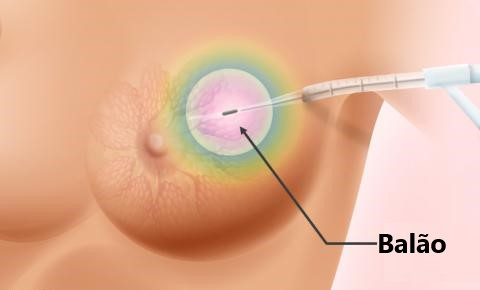
\includegraphics[width=0.8\textwidth]{Imagens/esquemaBalaoMama.jpg}
				\caption{Esquema de um tratamento de Braquiterapia de Mama utilizando um balão como aplicador.}
				\label{img:esquemaBalao}
			\end{figure}


			Em situações onde o PTV está próximo da pele ou da parede toráxica, é exigida uma assimetrida na distribuição de dose que só é alcançada comprometendo a dose no alvo (PTV), perdendo cobertura de dose no alvo ou aumentando as doses nos Orgãos de Risco (OARs).


			A prescrição de dose é feita a 1 cm do balão, portanto o raio do balão irá influenciar na dose na superfície do balão e consequentemente no gradiente de dose na região do alvo. Um balão com um diâmetro de 4.5 cm tem em sua superfície uma dose de aproximadamente 200\% da dose prescrita; quanto maior o diâmetro do balão, menor a dose na superfície do balão e vice-versa;

			A sutil anisotropia ao longo da direção do fio que conduz a fonte para as posições de parada pode ser suavizada utilizando múltiplos tempos de parada (carregamento não uniforme). 

			Em teoria, quanto maior o diâmetro do balão, mais uniforme será a dose no PTV, pois a região de tratamento será deslocada para uma região de menor gradiente de dose. No entanto, alguns centros reportaram uma maior incidência na formação de seromas e cecroses gordurosas ao utilizar balões com maiores volumes preenchidos.

			O plano de tratamento é feito com o balão inflado e portanto é importante avaliar o estado do balão antes de cada fração para evitar superdosagem no alvo. Esta avaliação pode ser realizada através de imagens de ultrasonografia, fluoroscopia ou Tomografia Computadorizada.

			Os balões multi-lumen foram desenvolvidos para contornar o problema obtido com os balões com um único lumen central: Proteger os OARs sem comprometer a cobertura do PTV. Exemplos dos balões Multi-lumens são o ConturaMLB e o MammoSiteML. Ambos mativeram o lumen central mas adicionaram lumens extras deslocados a prtir do centro. 

			A maior vantagem em utilizar dispositivos multi-lumen está do desacoplamento da cobertura do alvo com a proteção dos órgãos de risco que é inevitável utilizando apenas um lumen central. Com os balões Multi-lumen é possível criar distribuições de dose assimétricas que conformam melhor os PTV's assimétricos. Porém ao criar uma distribuição de dose assimétrica a partir de um balão simétrico, será criada regiões de dose dentro do volume alvo recebendo uma dose de radiação maior que a dose de prescrição.

			Os 3 balões\footnote{Ambos são comercializados pela empresa: Hologic Inc., Bedford, MA} mais utilizados são descritos abaixo:
			
			\begin{itemize}
				\item \textbf{\textcolor{DarkTurquoise}{MammoSite}}
				
					A    \ref{img:mammosite} mostra o balão e seus componentes. Este aplicador é constituído por um balão de silicone conectado por uma haste; possui um único lúmen por onde passa a fonte HDR e está disponível em dois tamanhos: 4.0 - 5.0 cm e 5.0 - 6.0 cm.

					\begin{figure}[h]
						\centering
						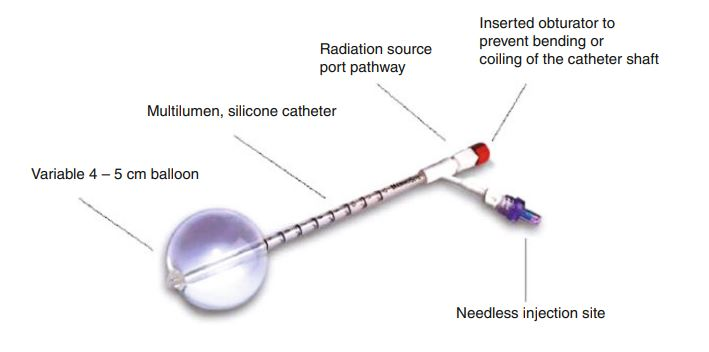
\includegraphics[width=0.4\textwidth]{Imagens/balaoMammoSite.JPG}
						\caption{MammoSite}
						\label{img:mammosite}
					\end{figure}

				\item \textbf{\textcolor{DarkTurquoise}{MammoSiteML}}
				
					A    \ref{img:mammositeml} mostra o balão e seus componentes. Este aplicador está disponível no tamanho de 3.5 - 5.0 cm e possui 4 lumens, sendo 1 lumen central e 3 lumens periférficos distibuídos em forma triangular à 0.3 cm do lúmen central.

					\begin{figure}[h]
						\centering
						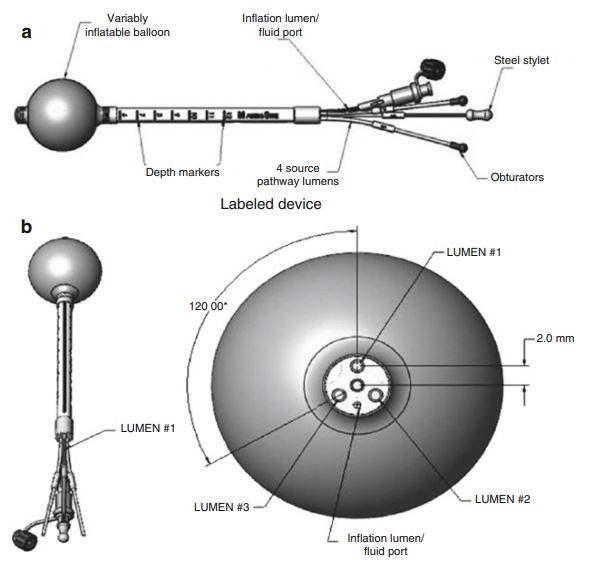
\includegraphics[width=0.4\textwidth]{Imagens/mammositeML.JPG}
						\caption{MammoSiteML}
						\label{img:mammositeml}
					\end{figure}

				
				\item \textbf{\textcolor{DarkTurquoise}{ConturaMLB}}
					
					A    \ref{img:conturaMLB} mostra os componentes deste aplicador. Está disponível nos tamanhos de 4 - 5 cm e 4.5 - 6 cm. Possui 5 lumens sendo 1 lumen central e outros 4 lumens periféricos igualmente espaçados a 0.5 cm de dustância do lúmem central. Possui duas portas de vácuo, nas partes proximal e distal do balão, que podem ser utilizadas para a remoção de ar ou fluido, aumentando a conformidade do tecido com a superfície do balão.
					
					\begin{figure}[h]
						\centering
						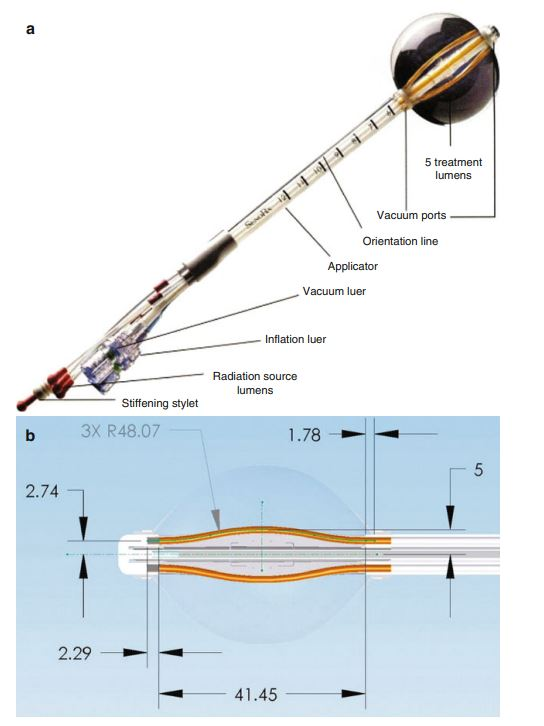
\includegraphics[width=0.4\textwidth]{Imagens/conturaMLB.JPG}
						\caption{ConturaMLB}
						\label{img:conturaMLB}
					\end{figure}
				\end{itemize}
			
			Os balões são inflados com uma solução salina e uma pequena quantidade de contraste para melhorar sua visualização. E para cada dispositivo é oferecido um balão para a avaliação do tamanho da cavidade, \textcolor{MediumOrchid}{Cavity Evaluation Device (CED)} que deve ser colocado no momento da mastectomia e somente no momento de tratamento ele é substituído por um balão de tratamento.

			Outo aplicador disponível no mercado é chamado de \textcolor{MediumOrchid}{Axxent}, que se trata de um balão desenvolvido com a braquiterapia eletrônica de 50 KeV (Xoft, Inc., Sunnyvale, CA) e semelhantemente ao MammoSite, possui apenas um único lumen central (\ref{img:axxent}).

			\begin{figure}[h]
				\centering
				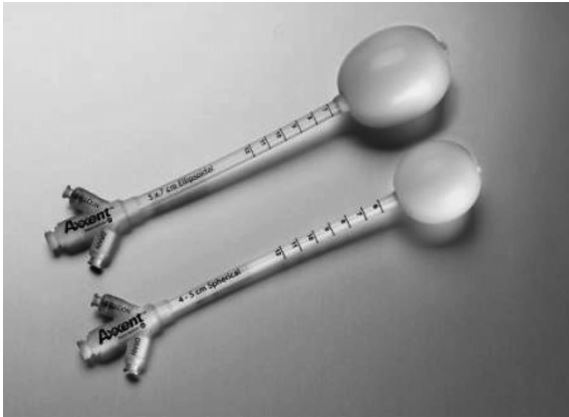
\includegraphics[width=0.45\textwidth]{Imagens/axxent.JPG}
				\caption{Aplicador Axxent}
				\label{img:axxent}
			\end{figure}

		








	\pagebreak
	\bibliography{ref.bib}

\end{document}